%QQQ Below: "10pt" prints in 10-point. "12pt" prints in larger 12-point.
\documentclass[12pt,letterpaper]{article}
\usepackage{amsthm,amssymb,amsmath}
\usepackage[pdftex]{hyperref}
\usepackage{tikz}
\usepackage{subcaption}
\usepackage{adjustbox}
%QQQ To print single-spaced, comment out the line below (precede it with a "%").
%QQQ To print double-spaced, remove the "%" at the beginning of the line.
%\renewcommand{\baselinestretch}{2}

% TIKZ

\pgfdeclarelayer{bg}    % declare background layer
\pgfsetlayers{bg,main}  % set the order of the layers

\tikzset{every label/.append style={fill=white}}
\tikzset{
    every node/.style={circle, inner sep=0mm, draw, minimum size=5mm, scale=.65}
}
\tikzset{every label/.style={shape=rectangle, draw=none, fill=white}}

% MARGINS

\setlength{\textwidth}{6.3in}
\setlength{\textheight}{8.7in}
\setlength{\topmargin}{0pt}
\setlength{\headsep}{0pt}
\setlength{\headheight}{0pt}
\setlength{\oddsidemargin}{0pt}
\setlength{\evensidemargin}{0pt}

% SET UP SECTION NUMBERING

\setcounter{secnumdepth}{1}
% Number sections, but not subsections

% BREAK THEOREM STYLE

\newtheoremstyle{break}% name
  {}%         Space above, empty = `usual value'
  {}%         Space below
  {}% Body font
  {}%         Indent amount (empty = no indent, \parindent = para indent)
  {\bfseries}% Thm head font
  {.}%        Punctuation after thm head
  {\newline}% Space after thm head: \newline = linebreak
  {}%         Thm head spec

% DEFINE THEOREM-LIKE STRUCTURES

\theoremstyle{plain}
\newtheorem{lemma}{Lemma}[section]           % L:
%\newtheorem{lemma}{Lemma}                    % L:
\newtheorem{proposition}[lemma]{Proposition} % P:
\newtheorem{theorem}[lemma]{Theorem}         % T:
\newtheorem{corollary}[lemma]{Corollary}     % C:
\newtheorem{conjecture}[lemma]{Conjecture}   % J:
\newtheorem{question}[lemma]{Question}       % Q:
\newtheorem{problem}[lemma]{Problem}         % B:

\newtheorem{observation}[lemma]{Observation} % O:
\newtheorem{remark}[lemma]{Remark}           % R:

\theoremstyle{definition}
\newtheorem{definition}[lemma]{Definition}   % D:
\newtheorem{example}[lemma]{Example}         % E:

\theoremstyle{break}
\newtheorem{algorithm}[lemma]{Algorithm}     % A:
\newtheorem{implementation}[lemma]{Implementation}     % A:

% Also: Section = S:, Figure = Fig:, Item = It:, Equation = Eq:

% CHANGE APPEARANCE OF ENUMERATED LISTS

\renewcommand{\labelenumi}{(\roman{enumi})} % Labels (i), (ii), etc.

% CHANGE QED-RELATED COMMANDS

\renewcommand{\qed}{}
\newcommand{\ggcqedsymbol}{$\square$}
\newcommand{\ggcqed}{\hbox{}\nobreak\hbox{\quad\ggcqedsymbol}}
\newcommand{\ggcendpf}{\ggcqed}
%\newcommand{\ggcnopf}{}
\newcommand{\ggcnopf}{\ggcqed}
%\newcommand{\ggcendexample}{}
\newcommand{\ggcendexample}{\ggcqed}

% SET STYLE FOR DEFINED TERMS

\newcommand{\defterm}[1]{\emph{#1}} % Defined term
\newcommand{\abstdefterm}[1]{#1} % Defined term in abstract
\newcommand{\localdefterm}[1]{\emph{#1}} % Defined term used only nearby

% RUN-IN HEADINGS

\newcommand{\runinhead}[1]{\vskip0.1in\textbf{#1}} % Run-in heading
% This should be used at the start of a paragraph,
%  with no space between it and the first word of the paragraph.

% DEFINITIONS SPECIFIC TO THIS DOCUMENT

% (NONE)

\date{June 1, 2017}

\title{Path-Coloring Algorithms for Plane Graphs}

\author{Aven Bross\\
\small Department of Computer Science\\
\small University of Alaska\\
\small Fairbanks, AK 99775-6670\\
\small\texttt{dabross@alaska.edu} \and
Glenn G.~Chappell\\
\small Department of Computer Science\\
\small University of Alaska\\
\small Fairbanks, AK 99775-6670\\
\small\texttt{chappellg{@}member.ams.org} \and
Chris Hartman\\
\small Department of Computer Science\\
\small University of Alaska\\
\small Fairbanks, AK 99775-6670\\
\small\texttt{cmhartman{@}alaska.edu}}

\begin{document}

\maketitle
\centerline{\small \textit{2010 Mathematics Subject Classification.}
 Primary 05C38; Secondary 05C10, 05C15.}
\centerline{\small \textit{Key words and phrases.}
 Path coloring, list coloring, algorithm.}

\begin{abstract}
A \abstdefterm{path coloring} of a graph $G$ is a vertex coloring
of $G$ such that each color class induces a disjoint union of paths.
We present two efficient algorithms
to construct a path coloring of a plane graph.

The first algorithm, based on a proof of Poh, %\cite{Poh1990}
is given a plane graph;
it produces a path coloring of the given graph
using three colors.

The second algorithm,
based on similar proofs
by Hartman % \cite{Har1997}
and \v{S}krekovski, %\cite{Skr1999}
performs a list-coloring generalization of the above.
The algorithm is given a plane graph and an assignment of lists of
three colors to each vertex;
it produces a path coloring of the given graph
in which each vertex receives a color from its list.

Implementations of both algorithms are available.
\end{abstract}


\section{Introduction}

All graphs will be finite, simple, and undirected.
See West~\cite{Wes2000} for graph theoretic terms.

A \defterm{path coloring} of a graph $G$ is a vertex coloring
(not necessarily proper) of $G$ such that each color class induces
a disjoint union of paths.
A graph $G$ is \defterm{path $k$-colorable} if $G$
admits a path coloring using $k$ colors.

Broere \& Mynhardt conjectured~\cite[Conj.~16]{BrMy1985}
that every planar graph is path $3$-colorable.
This was proven independently by Poh~\cite[Thm.~2]{Poh1990}
and by Goddard~\cite[Thm.~1]{God1991}.

\begin{theorem}[Poh 1990, Goddard 1991]\label{T:planar3c}
If $G$ is a planar graph,
then $G$ is path $3$-colorable.\ggcnopf\end{theorem}

It is easily shown that the ``$3$'' in Theorem~\ref{T:planar3c}
is best possible.
In particular, Chartrand \& Kronk~\cite[Section~3]{ChKr1969}
gave an example of a planar graph whose vertex set cannot be partitioned
into two subsets, each inducing a forest.

Hartman~\cite[Thm.~4.1]{Har1997}
proved a list-coloring generalization of Theorem~\ref{T:planar3c}
(see also Chappell \& Hartman~\cite[Thm.~2.1]{ChHa2017prep}).
A graph $G$ is \defterm{path $k$-choosable} if,
whenever each vertex of $G$ is assigned a list of $k$ colors,
there exists a path coloring of $G$ in which each vertex receives
a color from its list.

\begin{theorem}[Hartman 1997]\label{T:planar3}
If $G$ is a planar graph,
then $G$ is path $3$-choosable.\ggcnopf\end{theorem}

Essentially the same technique was used by
\v{S}krekovski~\cite[Thm.~2.2b]{Skr1999}
to prove a result slightly weaker than Theorem~\ref{T:planar3}.


\medskip

We discuss two efficient path-coloring algorithms
based on proofs of the above theorems.
We distinguish between a \defterm{planar} graph---one that
can be drawn in the plane without crossing edges---and
a \defterm{plane} graph---a graph with a given embedding
in the plane.

In Section~2 we outline our graph representations
and the basis for our computations of time complexity.

Section~3 covers an algorithm
based on Poh's proof of Theorem~\ref{T:planar3c}.
The algorithm is given a plane graph;
it produces a path coloring of the given graph
using three colors.

Section~4 covers an algorithm
based Hartman's proof of Theorem~\ref{T:planar3},
along with the proof of \v{S}krekovski mentioned above.
The algorithm is given a plane graph
and an assignment of a list of three colors to each vertex;
it produces a path coloring of the given graph
in which each vertex receives a color from its list.

Section~5 provides expiremental benchmarks for implementations of both
algorithms~\cite{Bro2017}. It also
discusses how both algorithms may be modified to benefit from parallelism.

\section{Graph Representations and Time Complexity}

We will represent a graph via \textit{adjacency lists}:
a list, for each vertex $v$, of the neighbors of $v$.
A vertex can be represented by an integer $0\dots n-1$,
where $n=n(G)$ is the order of the graph.

A plane graph will be specified via
a \defterm{rotation scheme}:
a circular ordering,
for each vertex $v$, of the edges incident with $v$,
in the order they appear around $v$ in the plane embedding;
this completely specifies
the combinatorial embedding of the graph.
Rotation schemes are convenient when we represent a graph
using adjacency lists;
we simply order the adjacency
list for each vertex $v$ in clockwise order around $v$;
no additional data structures are required.

We will assume that both forward and backward iteration in adjacency lists
is constant time. In terms of plane graphs: given the entry for an edge in a
rotation scheme ordered adjacency list, we assume that it is a
constant time operation to retrieve entries corresponding to the
immediately clockwise and counter-clockwise edges. The provided
C implementation uses adjacency arrays, but a doubly linked list
would also suffice.

The input for each algorithm will be a weakly triangulated plane graph with
$n$ vertices and $m$ edges, represented
via adjacency lists. The input size will be $n$, the number of vertices. Note
that $\mathcal{O}(m)=\mathcal{O}(n)$, so it is equivalent to take the input size
to be $m$, the number of edges. Moreover, arbitrary simple planar graphs may be
plane embedded and triangulated in $\mathcal{O}(n)$ time, see Boyer and
Myrvold~\cite{BoMy2004}.

In Section~4, given an edge $uv$, we will need an efficient operation to
find $v$'s entry in $u$'s adjacency list from $u$'s entry in $v$'s list.
We define an \defterm{augmented adjacency list} to be an adjacency list such
that for
every edge $uv$ a reference to $v$'s entry in
$u$'s list is stored in $u$'s entry in $v$'s list, and vice versa. Given an
adjacency list representation of a graph, an augmented
adjacency list representation may be constructed in $\mathcal{O}(m)$ time via
the following procedure.

\begin{algorithm}\label{A:augment}
\textbf{Input:} An adjacency list representation Adj of a graph $G$.

\textbf{Output:} An augmented adjacency list representation AugAdj of
$G$ with the same rotation scheme as Adj.

\textbf{Step 1:} Construct an augmented adjacency list AugAdj with
the same rotation scheme as Adj leaving the reference portion of each entry
uninitialized.

\textbf{Step 2:} For each vertex $v$ construct an array $\text{Wrk}[v]$
of vertex-reference pairs with length $\text{deg}(v)$. For each $v$ from
$0$ to $n-1$ iterate through
$\text{AugAdj}[v]$. For each neighbor $u$ in $\text{AugAdj}[v]$ append the pair
$(v,r_v(u))$ to
$\text{Wrk}[u]$, where $r_v(u)$ is a reference to $u$'s entry in
$\text{AugAdj}[v]$.

\textbf{Step 3:} For each $v$ from $n-1$ to $0$ iterate through
$\text{Wrk}[v]$. Upon reaching a pair $(u,r_u(v))$ in $\text{Wrk}[v]$ the
last element of $\text{Wrk}[u]$ will be $(v,r_v(u))$; for details on why this
must be the case, see the paragraph below. Use
$r_u(v)$ and $r_v(u)$ to look up and assign references for the edge $uv$ in
AugAdj$[u]$ and AugAdj$[v]$. Remove $(v,r_v(u))$ from the back of
$\text{Wrk}[u]$.
\end{algorithm}

After completing Step $2$ in Algorithm~\ref{A:augment} the array $\text{Wrk}[v]$
will contain
a pair $(u,r_u(v))$ for each neighbor $u$ of $v$, sorted in increasing order by
the neighbor $u$.
Suppose that $v$ is the current vertex at a given iteration of Step $3$ in
Algorithm~\ref{A:augment}. For each edge $uw\in E(G)$ such that
$u<w$ and $v<w$, prior iterations of Step 3 will have initialized the
references for $uw$ in $\text{AugAdj}[u]$ and $\text{AugAdj}[w]$, and also
removed the pair
$(w,r_w(u))$ from $\text{Wrk}[u]$. Therefore for each $(u,r_u(v))$ in
$\text{Wrk}[v]$, the array $\text{Wrk}[u]$ will contain only entries for
vertices $w$ where $w\le v$. Since $\text{Wrk}[u]$ is sorted in
increasing order by the neighboring vertices, the last element of
$\text{Wrk}[u]$ must be $(v,r_v(u))$.

\section{Path Coloring: the Poh Algorithm}

We will first describe Poh's path $3$-coloring algorithm.
Given a cycle $C$ in a plane graph $G$ we define $\text{Int}(C)$ to
be the subgraph of $G$ consisting of $C$ and all vertices and edges interior to
$C$. Equivalently, $\text{Int}(C)$ is the maximal subgraph of $G$ which has
outer face $C$.

\begin{algorithm}[Poh 1990]\label{A:planar3}
\textbf{Input:} Let $G$ be a weakly triangulated plane graph with outer face a
cycle $C=v_1,v_2,\ldots, v_k$. Let $c$ be a $2$-coloring of $C$ such
that each color class induces a path, $P_1=v_1,v_2,\ldots, v_\ell$ and
$P_2=v_{l+1},v_{l+2},\ldots, v_k$ respectively.

\textbf{Output:} An extension of the $2$-coloring $c$ of $C$ to a path
$3$-coloring of $G$ such that no vertex in $G-C$ receives the same color as a
neighbor of that vertex in $C$.

\textbf{Step 1:} If $G=C$ then $G$ is already path $3$-colored and we
are done. Otherwise there are two cases to consider.

\textbf{Case 1.1:} Suppose $C$ is an induced subgraph of $G$. Let
$u,w\in V(G)-V(C)$ such that the cycles $u,v_1,v_k$ and $w,v_\ell,v_{\ell+1}$ each
exist and are faces of $G$; note that
$u$ and $w$ are uniquely determined, but it may be the case that $u=w$. Since
$C$ is an induced cycle in $G$ and
$G\ne C$, $G-C$ is connected.
Let $P_3=u_1,u_2,\ldots,u_r$ be an induced $u,w$-path in $G-C$.
Color each vertex of $P_3$ with the third color not used in the $2$-coloring of
$C$. Let $C_1=v_1,v_2,\ldots,v_\ell,u_r,u_{r-1},\ldots,u_1$ and
$C_2=u_1,u_2,\ldots,u_r,v_{\ell+1},v_{l+2},\ldots,v_k$.

\textbf{Case 1.2:} Suppose $C$ is not an induced subgraph. Then there
exists an edge $v_iv_j\in E(G)-E(C)$ such that $i\le \ell < j$. Let
$C_1=v_1,v_2,\ldots,v_i,v_j,v_{j+1},\ldots,v_k$
and $C_2=v_i,v_{i+1},\ldots,v_j$.

\textbf{Step 2:} Apply Algorithm~\ref{A:planar3} separately to $\text{Int}(C_1)$
and $\text{Int}(C_2)$. The resulting path $3$-colorings agree and extend to
a path $3$-coloring of $G$. 
\end{algorithm}

\begin{figure}[h]
\begin{center}
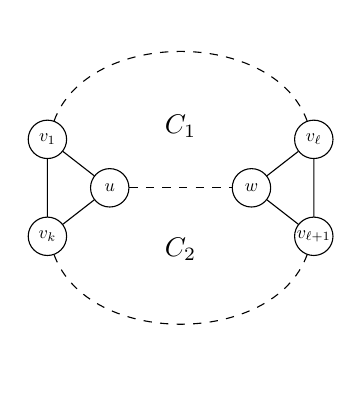
\begin{tikzpicture}[scale=1.2]
    \node (p0)[minimum size=7.5mm] at (160:1.5cm) {$v_1$};
  \node (pn) [minimum size=7.5mm] at (20:1.5cm) {$v_\ell$};
  \node (q0) [minimum size=7.5mm] at (200:1.5cm) {$v_k$};
    \node (qn) [minimum size=7.5mm] at (340:1.5cm) {$v_{\ell+1}$};
  \node (t0) [minimum size=7.5mm] at (180:0.75cm) {$u$};
  \node (t1) [minimum size=7.5mm] at (0:0.75cm) {$w$};
    \node (null) [draw=none, fill=none] at (270:1.75cm) {};
  
  \node (C1) [scale=1.5] [draw=none, fill=none] at (90:0.65cm) {$C_1$};
  \node (C2) [scale=1.5] [draw=none, fill=none] at (270:0.65cm) {$C_2$};
  
  \draw (p0) edge [bend left=70] (pn) [dashed];
  \draw (q0) edge [bend right=70] (qn) [dashed];
  \draw (p0) edge (q0);
  \draw (pn) edge (qn);
  \draw (p0) edge (t0);
  \draw (q0) edge (t0);
  \draw (pn) edge (t1);
  \draw (qn) edge (t1);
  \draw (t0) edge (t1) [dashed];
\end{tikzpicture}
$\qquad$
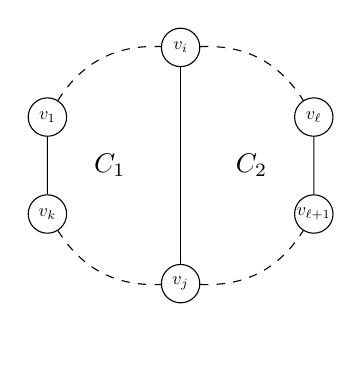
\begin{tikzpicture}[scale=1.2]
  \node (p0) [minimum size=7.5mm] at (160:1.5cm) {$v_1$};
  \node (p1) [minimum size=7.5mm] at (90:1.25cm) {$v_i$};
  \node (pn) [minimum size=7.5mm] at (20:1.5cm) {$v_\ell$};
  \node (q0) [minimum size=7.5mm] at (200:1.5cm) {$v_k$};
  \node (q1) [minimum size=7.5mm] at (270:1.25cm) {$v_j$};
    \node (qn) [minimum size=7.5mm] at (340:1.5cm) {$v_{\ell+1}$};
  \node (null) [draw=none, fill=none] at (270:1.75cm) {};
  
    \node (C1) [scale=1.5] [draw=none, fill=none] at (180:0.75cm) {$C_1$};
    \node (C2) [scale=1.5] [draw=none, fill=none] at (0:0.75cm) {$C_2$};
  
  \draw (p0) edge [bend left] (p1) [dashed];
  \draw (p1) edge [bend left] (pn) [dashed];
  \draw (q0) edge [bend right] (q1) [dashed];
  \draw (q1) edge [bend right] (qn) [dashed];
  \draw (p0) edge (q0);
  \draw (pn) edge (qn);
  \draw (p1) edge (q1);
\end{tikzpicture}
\caption{Algorithm~\ref{A:planar3} Case 1.1 (left) and Case 1.2 (right).}
\label{poh_figure}
\end{center}
\end{figure}

Note that the graph $G$ is finite and the recursive
step applies the algorithm to two proper subgraphs of $G$. Therefore
Algorithm~\ref{A:planar3} must terminate.

Let $G$ be a triangulated plane graph. We may trivially path $2$-color the outer
triangle. Applying Poh's algorithm extends this coloring to a path $3$-coloring
of $G$.

In Poh's original proof he picked the induced $u,w$-path in Case 1.1 to be the
shortest $u,w$-path.
Thus a natural way to implement Poh's algorithm is to first locate $u$ and $w$,
and then use a breadth-first search to
to either construct a $u,w$-path or locate
a chord edge if no such path is possible.

\begin{algorithm}\label{A:poh_bfs}
\textbf{Input:} Let $C=v_1,v_2,\ldots,v_k$ be a cycle in a weakly triangulated plane
graph $G$ with adjacency list representation $\text{Adj}$. Let 
$c$ be an array of colors repreenting a $2$-coloring of $C$ such
that each color class induces a single path, respectively labelled
$P_1=v_1,v_2,\ldots,v_\ell$ and $P_2=v_\ell,v_{\ell+1},\ldots,v_k$. Assume that
$c[v]=0$ for all $v\in\text{Int}(C)-C$.

\textbf{Output:} Each vertex $v\in\text{Int}(C)-C$ a nonzero color will be
assigned to $c[v]$ such that $c$ represents a path $3$-coloring of
$\text{Int}(C)$ extending the original $2$-coloring of $C$.

\textbf{Step 1:} Iterate through $\text{Adj}[v_\ell]$ to locate the vertex $u$
immediately following $v_k$. Note that since $G$ is triangulated, $v_1,u,v_k$ is
a face of $G$.

\textbf{Case 1.1:} If $u\in C$, then $u=v_{k-1}$, since $G$ is
triangulated, and $C$ is not an induced cycle. We then
apply Algorithm~\ref{A:poh_bfs} to the cycle $C'=v_1,v_2,\ldots,v_{k-1}$.

\textbf{Case 1.2:} Perform a breadth-first of the maximal subgraph of
$G$ with outer face $C$, starting from the
vertex $u$. Terminate the search upon locating a vertex $w\not\in C$ with adjacent
neighbors $v_i\in P_1$ and $v_j\in P_2$ such that $i\ne 1$ or $j\ne k$.
Backtrack along the breadth-first search
to construct a minimal $u,w$-path $P_3=u_1,u_2,\ldots,u_r$. Let
$C_1=v_1,v_2,\ldots,v_i,u_r,u_{r-1},\ldots,u_1$ and
$C_2=u_1,u_2,\ldots,u_r,v_j,v_{j-1},\ldots,v_k$. Apply Algorithm~\ref{A:poh_bfs}
separately to $C_1$ and $C_2$. If $i=l$ and $j={\ell+1}$ then $C$ was an induced
cycle and we are done. Otherwise, also apply Algorithm~\ref{A:poh_bfs} to
$C_3=v_i,v_{i+1},\ldots,v_j$.
\end{algorithm}

\begin{figure}[h]
\begin{center}
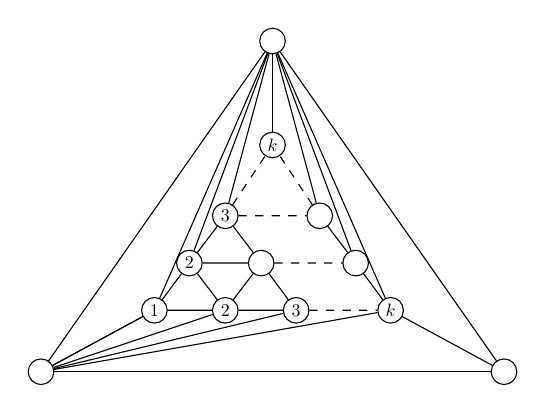
\begin{tikzpicture}[scale=1.2]
  \node (t1) at (0cm, 3.5cm) {};
  \node (t2) at (2.45cm, 0cm) {};
  \node (t3) at (-2.45cm, 0cm) {};

  \node (k1) at (-1.25cm, 0.65cm) {$1$};
  \node (k2) at (-0.5cm, 0.65cm) {$2$};
  \node (k3) at (0.25cm, 0.65cm) {$3$};
  \node (kn) at (1.25cm, 0.65cm) {$k$};

  \node (l1) at (-0.88cm, 1.15cm) {$2$};
  \node (l2) at (-0.12cm, 1.15cm) {};
  \node (ln) at (0.88cm, 1.15cm) {};

  \node (j1) at (-0.5cm, 1.65cm) {$3$};
  \node (jn) at (0.5cm, 1.65cm) {};

  \node (p) at (0cm, 2.4cm) {$k$};

  \begin{pgfonlayer}{bg}
	  \draw (t1) edge (t2); \draw (t3) edge (t2); \draw (t1) edge (t3);
	  \draw (k1) edge (k2); \draw (k3) edge (k2);
	  \draw (k3) edge (kn) [dashed];

	  \draw (l1) edge (l2);
	  \draw (l2) edge (ln) [dashed];

	  \draw (j1) edge (jn) [dashed];

	  \draw (j1) edge (p) [dashed];
	  \draw (jn) edge (p) [dashed];

	  \draw (t1) edge (k1); \draw (t1) edge (kn);
	  \draw (t1) edge (l1); \draw (t1) edge (ln);
	  \draw (t1) edge (p);
	  \draw (t2) edge (kn); \draw (t3) edge (k1);

	  \draw (k1) edge (l1); \draw (k2) edge (l1);
	  \draw (k2) edge (l2); \draw (k3) edge (l2);
	  \draw (kn) edge (ln);

	  \draw (l1) edge (j1); \draw (l2) edge (j1);
	  \draw (jn) edge (ln);

	  \draw (j1) edge (t1); \draw (jn) edge (t1);

	  \draw (t3) edge (k1); \draw (t3) edge (k2);
	  \draw (t3) edge (k3); \draw (t3) edge (kn);
  \end{pgfonlayer}

\end{tikzpicture}

\caption{The collection of graphs $\{G_k\}_{k\in\mathbb{N}}$ on which Poh
performs poorly.}\label{F:poh_bad_graph_collection}
\end{center}
\end{figure}

Unfortunately Algorithm~\ref{A:poh_bfs}
is not linear. Consider the family of
graphs $\{G_k\}_{k\in\mathbb{N}}$ depicted in
Figure~\ref{F:poh_bad_graph_collection}. Fix $k\in\mathbb{N}$ and note that
$n=n(G_k)=k(k+1)/2+3$. Assume
that the outer triangle is path $2$-colored such that the top vertex is
assigned a color distinct from the bottom two. At iteration $i$ of Poh's
algorithm the shortest path through the interior will be the path of length
$r=k-i+1$ directly along the base of the inner triangle. A breadth-first search
of this inner triangle will hit all $r(r+1)/2$ vertices in order to find this
path. Therefore the total number of operations performed will be
\[
    \Theta\left( \sum_{r=1}^k\frac{r(r+1)}{2} \right)=\Theta(n^{3/2}).
\]
So Poh's algorithm with breadth-first search is $\Omega(n^{3/2})$.

However, the correctness of Poh's algorithm only relied on
locating some induced $u,w$-path.
We will show below that there exists a linear time implementation of Poh's
algorithm so long as we do not always find the shortest $u,w$-path.

Let $N(P_1)$ be the set of vertices with a neighbor in $P_1$. The
strategy will be to construct a
path $P_3=u_1,u_2,\ldots,u_d$ consisting of vertices in $N(P_1)$
such that $C_1=P_1\cup P_3\cup\{u_1v_1,u_dv_l\}$ is a cycle of minimal length.

\begin{figure}[h]
\begin{center}
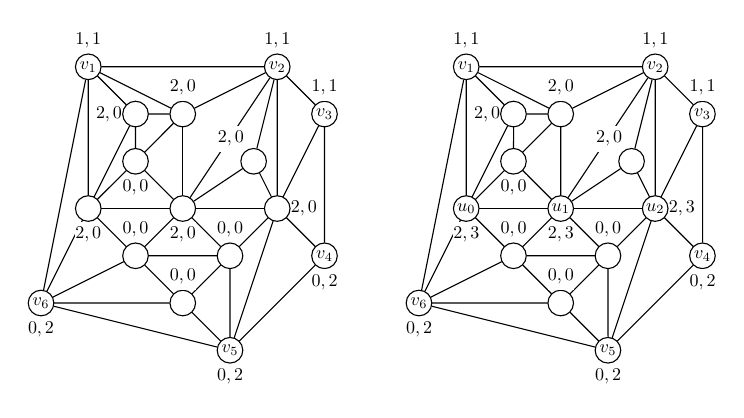
\begin{tikzpicture}[scale=1.2]
    \node (v1) [label=above:${1,1}$] at (-1cm, 1.5cm) {$v_1$};
    \node (v2) [label=above:${1,1}$] at (1cm, 1.5cm) {$v_2$};
    \node (v3) [label=above:${1,1}$] at (1.5cm, 1.0cm) {$v_3$};
    \node (v4) [label=below:${0,2}$] at (1.5cm, -0.5cm) {$v_4$};
    \node (v5) [label=below:${0,2}$] at (0.5cm, -1.5cm) {$v_5$};
    \node (v6) [label=below:${0,2}$] at (-1.5cm, -1.0cm) {$v_6$};

    \node (u1) [label=below:${2,0}$] at (-1cm, 0.0cm) {};
    \node (u2) [label=below:${2,0}$] at (0.0cm, 0.0cm) {};
    \node (u3) [label=right:${2,0}$] at (1cm, 0.0cm) {};

    \node (p1) [label=left:${2,0}$] at (-0.5cm, 1.0cm) {};
    \node (p2) [label=above:${2,0}$] at (0.0cm, 1.0cm) {};
    \node (p3) [label=below:${0,0}$] at (-0.5cm, 0.5cm) {};
    \node (p4) [label=above left:${2,0}$] at (0.75cm, 0.5cm) {};

    \node (q1) [label=above:${0,0}$] at (-0.5cm, -0.5cm) {};
    \node (q2) [label=above:${0,0}$] at (0.5cm, -0.5cm) {};
    \node (q3) [label=above:${0,0}$] at (0.0cm, -1.0cm) {};

    \begin{pgfonlayer}{bg}
        \draw (v1) edge (v2);
        \draw (v2) edge (v3);
        \draw (v3) edge (v4);
        \draw (v4) edge (v5);
        \draw (v5) edge (v6);
        \draw (v6) edge (v1);

        \draw (v1) edge (u1);
        \draw (v6) edge (u1);
        \draw (v2) edge (u2);
        \draw (v2) edge (u3);
        \draw (v3) edge (u3);
        \draw (v4) edge (u3);
        \draw (v5) edge (u3);

        \draw (v1) edge (p1);
        \draw (v1) edge (p2);
        \draw (v2) edge (p2);
        \draw (v2) edge (p4);

        \draw (v5) edge (q3);
        \draw (v5) edge (q2);
        \draw (v6) edge (q1);
        \draw (v6) edge (q3);

        \draw (u1) edge (p1);
        \draw (u1) edge (p3);
        \draw (u2) edge (p2);
        \draw (u2) edge (p3);
        \draw (u2) edge (p4);
        \draw (u3) edge (p4);

        \draw (u1) edge (q1);
        \draw (u2) edge (q1);
        \draw (u2) edge (q2);
        \draw (u3) edge (q2);

        \draw (u1) edge (u2);
        \draw (u2) edge (u3);

        \draw (p1) edge (p2);
        \draw (p1) edge (p3);
        \draw (p2) edge (p3);

        \draw (q1) edge (q2);
        \draw (q1) edge (q3);
        \draw (q2) edge (q3);
    \end{pgfonlayer}

    \node (v1b) [label=above:${1,1}$] at (3cm, 1.5cm) {$v_1$};
    \node (v2b) [label=above:${1,1}$] at (5cm, 1.5cm) {$v_2$};
    \node (v3b) [label=above:${1,1}$] at (5.5cm, 1.0cm) {$v_3$};
    \node (v4b) [label=below:${0,2}$] at (5.5cm, -0.5cm) {$v_4$};
    \node (v5b) [label=below:${0,2}$] at (4.5cm, -1.5cm) {$v_5$};
    \node (v6b) [label=below:${0,2}$] at (2.5cm, -1.0cm) {$v_6$};

    \node (u1b) [label=below:${2,3}$] at (3cm, 0.0cm) {$u_0$};
    \node (u2b) [label=below:${2,3}$] at (4.0cm, 0.0cm) {$u_1$};
    \node (u3b) [label=right:${2,3}$] at (5cm, 0.0cm) {$u_2$};

    \node (p1b) [label=left:${2,0}$] at (3.5cm, 1.0cm) {};
    \node (p2b) [label=above:${2,0}$] at (4.0cm, 1.0cm) {};
    \node (p3b) [label=below:${0,0}$] at (3.5cm, 0.5cm) {};
    \node (p4b) [label=above left:${2,0}$] at (4.75cm, 0.5cm) {};

    \node (q1b) [label=above:${0,0}$] at (3.5cm, -0.5cm) {};
    \node (q2b) [label=above:${0,0}$] at (4.5cm, -0.5cm) {};
    \node (q3b) [label=above:${0,0}$] at (4.0cm, -1.0cm) {};

    \begin{pgfonlayer}{bg}
        \draw (v1b) edge (v2b);
        \draw (v2b) edge (v3b);
        \draw (v3b) edge (v4b);
        \draw (v4b) edge (v5b);
        \draw (v5b) edge (v6b);
        \draw (v6b) edge (v1b);

        \draw (v1b) edge (u1b);
        \draw (v6b) edge (u1b);
        \draw (v2b) edge (u2b);
        \draw (v2b) edge (u3b);
        \draw (v3b) edge (u3b);
        \draw (v4b) edge (u3b);
        \draw (v5b) edge (u3b);

        \draw (v1b) edge (p1b);
        \draw (v1b) edge (p2b);
        \draw (v2b) edge (p2b);
        \draw (v2b) edge (p4b);

        \draw (v5b) edge (q3b);
        \draw (v5b) edge (q2b);
        \draw (v6b) edge (q1b);
        \draw (v6b) edge (q3b);

        \draw (u1b) edge (p1b);
        \draw (u1b) edge (p3b);
        \draw (u2b) edge (p2b);
        \draw (u2b) edge (p3b);
        \draw (u2b) edge (p4b);
        \draw (u3b) edge (p4b);

        \draw (u1b) edge (q1b);
        \draw (u2b) edge (q1b);
        \draw (u2b) edge (q2b);
        \draw (u3b) edge (q2b);

        \draw (u1b) edge (u2b);
        \draw (u2b) edge (u3b);

        \draw (p1b) edge (p2b);
        \draw (p1b) edge (p3b);
        \draw (p2b) edge (p3b);

        \draw (q1b) edge (q2b);
        \draw (q1b) edge (q3b);
        \draw (q2b) edge (q3b);
  \end{pgfonlayer}
\end{tikzpicture}
$\quad$
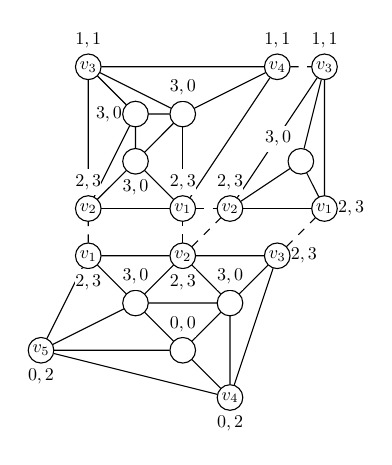
\begin{tikzpicture}[scale=1.2]
    \node (v1) [label=above:${1,1}$] at (-1cm, 1.5cm) {$v_3$};
    \node (v2) [label=above:${1,1}$] at (1cm, 1.5cm) {$v_4$};
    \node (u1) [label=above:${2,3}$] at (-1cm, 0.0cm) {$v_2$};
    \node (u2) [label=above:${2,3}$] at (0.0cm, 0.0cm) {$v_1$};
    \node (p1) [label=left:${3,0}$] at (-0.5cm, 1.0cm) {};
    \node (p2) [label=above:${3,0}$] at (0.0cm, 1.0cm) {};
    \node (p3) [label=below:${3,0}$] at (-0.5cm, 0.5cm) {};

    \node (v2r) [label=above:${1,1}$] at (1.5cm, 1.5cm) {$v_3$};
    \node (u2r) [label=above:${2,3}$] at (0.5cm, 0.0cm) {$v_2$};
    \node (u3r) [label=right:${2,3}$] at (1.5cm, 0.0cm) {$v_1$};
    \node (p4r) [label=above left:${3,0}$] at (1.25cm, 0.5cm) {};

    \node (u1s) [label=below:${2,3}$] at (-1cm, -0.5cm) {$v_1$};
    \node (u2s) [label=below:${2,3}$] at (0.0cm, -0.5cm) {$v_2$};
    \node (u3s) [label=right:${2,3}$] at (1cm, -0.5cm) {$v_3$};
    \node (v5s) [label=below:${0,2}$] at (0.5cm, -2.0cm) {$v_4$};
    \node (v6s) [label=below:${0,2}$] at (-1.5cm, -1.5cm) {$v_5$};
    \node (q1s) [label=above:${3,0}$] at (-0.5cm, -1.0cm) {};
    \node (q2s) [label=above:${3,0}$] at (0.5cm, -1.0cm) {};
    \node (q3s) [label=above:${0,0}$] at (0.0cm, -1.5cm) {};

    \begin{pgfonlayer}{bg}
        \draw (v1) edge (v2);
        \draw (v1) edge (u1);
        \draw (v2) edge (u2);
        \draw (v1) edge (p1);
        \draw (v1) edge (p2);
        \draw (v2) edge (p2);
        \draw (u1) edge (p1);
        \draw (u1) edge (p3);
        \draw (u2) edge (p2);
        \draw (u2) edge (p3);
        \draw (p1) edge (p2);
        \draw (p1) edge (p3);
        \draw (p2) edge (p3);
        \draw (u1) edge (u2);

        \draw (u2) edge [dashed] (u2r);
        \draw (v2) edge [dashed] (v2r);

        \draw (u2r) edge (u3r);
        \draw (u2r) edge (p4r);
        \draw (u3r) edge (p4r);
        \draw (v2r) edge (p4r);
        \draw (v2r) edge (u2r);
        \draw (v2r) edge (u3r);

        \draw (u1s) edge [dashed] (u1);
        \draw (u2s) edge [dashed] (u2);
        \draw (u2s) edge [dashed] (u2r);
        \draw (u3s) edge [dashed] (u3r);

        \draw (v5s) edge (v6s);
        \draw (u1s) edge (u2s);
        \draw (u2s) edge (u3s);
        \draw (v5s) edge (u3s);
        \draw (v6s) edge (u1s);
        \draw (u1s) edge (q1s);
        \draw (u2s) edge (q1s);
        \draw (u2s) edge (q2s);
        \draw (u3s) edge (q2s);
        \draw (v5s) edge (q3s);
        \draw (v5s) edge (q2s);
        \draw (v6s) edge (q1s);
        \draw (v6s) edge (q3s);
        \draw (q1s) edge (q2s);
        \draw (q1s) edge (q3s);
        \draw (q2s) edge (q3s);
    \end{pgfonlayer}
\end{tikzpicture}
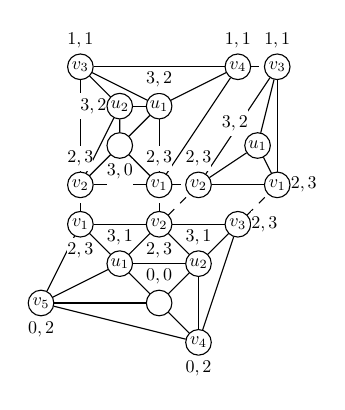
\begin{tikzpicture}
    \node (v1) [label=above:${1,1}$] at (-1cm, 1.5cm) {$v_3$};
    \node (v2) [label=above:${1,1}$] at (1cm, 1.5cm) {$v_4$};
    \node (u1) [label=above:${2,3}$] at (-1cm, 0.0cm) {$v_2$};
    \node (u2) [label=above:${2,3}$] at (0.0cm, 0.0cm) {$v_1$};
    \node (p1) [label=left:${3,2}$] at (-0.5cm, 1.0cm) {$u_2$};
    \node (p2) [label=above:${3,2}$] at (0.0cm, 1.0cm) {$u_1$};
    \node (p3) [label=below:${3,0}$] at (-0.5cm, 0.5cm) {};

    \node (v2r) [label=above:${1,1}$] at (1.5cm, 1.5cm) {$v_3$};
    \node (u2r) [label=above:${2,3}$] at (0.5cm, 0.0cm) {$v_2$};
    \node (u3r) [label=right:${2,3}$] at (1.5cm, 0.0cm) {$v_1$};
    \node (p4r) [label=above left:${3,2}$] at (1.25cm, 0.5cm) {$u_1$};

    \node (u1s) [label=below:${2,3}$] at (-1cm, -0.5cm) {$v_1$};
    \node (u2s) [label=below:${2,3}$] at (0.0cm, -0.5cm) {$v_2$};
    \node (u3s) [label=right:${2,3}$] at (1cm, -0.5cm) {$v_3$};
    \node (v5s) [label=below:${0,2}$] at (0.5cm, -2.0cm) {$v_4$};
    \node (v6s) [label=below:${0,2}$] at (-1.5cm, -1.5cm) {$v_5$};
    \node (q1s) [label=above:${3,1}$] at (-0.5cm, -1.0cm) {$u_1$};
    \node (q2s) [label=above:${3,1}$] at (0.5cm, -1.0cm) {$u_2$};
    \node (q3s) [label=above:${0,0}$] at (0.0cm, -1.5cm) {};

    \begin{pgfonlayer}{bg}
        \draw (v1) edge (v2);
        \draw (v1) edge (u1);
        \draw (v2) edge (u2);
        \draw (v1) edge (p1);
        \draw (v1) edge (p2);
        \draw (v2) edge (p2);
        \draw (u1) edge (p1);
        \draw (u1) edge (p3);
        \draw (u2) edge (p2);
        \draw (u2) edge (p3);
        \draw (p1) edge (p2);
        \draw (p1) edge (p3);
        \draw (p2) edge (p3);
        \draw (u1) edge (u2);

        \draw (u2) edge [dashed] (u2r);
        \draw (v2) edge [dashed] (v2r);

        \draw (u2r) edge (u3r);
        \draw (u2r) edge (p4r);
        \draw (u3r) edge (p4r);
        \draw (v2r) edge (p4r);
        \draw (v2r) edge (u2r);
        \draw (v2r) edge (u3r);

        \draw (u1s) edge [dashed] (u1);
        \draw (u2s) edge [dashed] (u2);
        \draw (u2s) edge [dashed] (u2r);
        \draw (u3s) edge [dashed] (u3r);

        \draw (v5s) edge (v6s);
        \draw (u1s) edge (u2s);
        \draw (u2s) edge (u3s);
        \draw (v5s) edge (u3s);
        \draw (v6s) edge (u1s);
        \draw (u1s) edge (q1s);
        \draw (u2s) edge (q1s);
        \draw (u2s) edge (q2s);
        \draw (u3s) edge (q2s);
        \draw (v5s) edge (q3s);
        \draw (v5s) edge (q2s);
        \draw (v6s) edge (q1s);
        \draw (v6s) edge (q3s);
        \draw (q1s) edge (q2s);
        \draw (q1s) edge (q3s);
        \draw (q2s) edge (q3s);
    \end{pgfonlayer}
\end{tikzpicture}
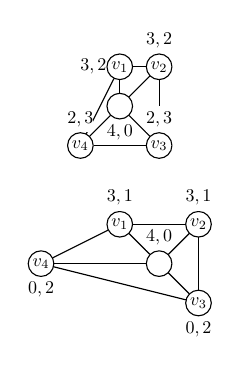
\begin{tikzpicture}
    \node (u1) [label=above:${2,3}$] at (-1cm, 0.0cm) {$v_4$};
    \node (u2) [label=above:${2,3}$] at (0.0cm, 0.0cm) {$v_3$};
    \node (p1) [label=left:${3,2}$] at (-0.5cm, 1.0cm) {$v_1$};
    \node (p2) [label=above:${3,2}$] at (0.0cm, 1.0cm) {$v_2$};
    \node (p3) [label=below:${4,0}$] at (-0.5cm, 0.5cm) {};

    \node (v5s) [label=below:${0,2}$] at (0.5cm, -2.0cm) {$v_3$};
    \node (v6s) [label=below:${0,2}$] at (-1.5cm, -1.5cm) {$v_4$};
    \node (q1s) [label=above:${3,1}$] at (-0.5cm, -1.0cm) {$v_1$};
    \node (q2s) [label=above:${3,1}$] at (0.5cm, -1.0cm) {$v_2$};
    \node (q3s) [label=above:${4,0}$] at (0.0cm, -1.5cm) {};

    \begin{pgfonlayer}{bg}
        \draw (u1) edge (p1);
        \draw (u1) edge (p3);
        \draw (u2) edge (p2);
        \draw (u2) edge (p3);
        \draw (p1) edge (p2);
        \draw (p1) edge (p3);
        \draw (p2) edge (p3);
        \draw (u1) edge (u2);

        \draw (v5s) edge (v6s);
        \draw (v5s) edge (q3s);
        \draw (v5s) edge (q2s);
        \draw (v6s) edge (q1s);
        \draw (v6s) edge (q3s);
        \draw (q1s) edge (q2s);
        \draw (q1s) edge (q3s);
        \draw (q2s) edge (q3s);
    \end{pgfonlayer}
\end{tikzpicture}
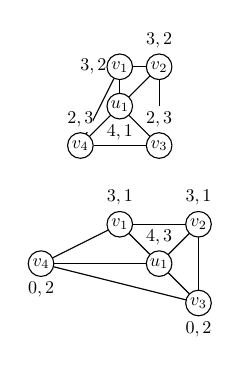
\begin{tikzpicture}
    \node (u1) [label=above:${2,3}$] at (-1cm, 0.0cm) {$v_4$};
    \node (u2) [label=above:${2,3}$] at (0.0cm, 0.0cm) {$v_3$};
    \node (p1) [label=left:${3,2}$] at (-0.5cm, 1.0cm) {$v_1$};
    \node (p2) [label=above:${3,2}$] at (0.0cm, 1.0cm) {$v_2$};
    \node (p3) [label=below:${4,1}$] at (-0.5cm, 0.5cm) {$u_1$};

    \node (v5s) [label=below:${0,2}$] at (0.5cm, -2.0cm) {$v_3$};
    \node (v6s) [label=below:${0,2}$] at (-1.5cm, -1.5cm) {$v_4$};
    \node (q1s) [label=above:${3,1}$] at (-0.5cm, -1.0cm) {$v_1$};
    \node (q2s) [label=above:${3,1}$] at (0.5cm, -1.0cm) {$v_2$};
    \node (q3s) [label=above:${4,3}$] at (0.0cm, -1.5cm) {$u_1$};

    \begin{pgfonlayer}{bg}
        \draw (u1) edge (p1);
        \draw (u1) edge (p3);
        \draw (u2) edge (p2);
        \draw (u2) edge (p3);
        \draw (p1) edge (p2);
        \draw (p1) edge (p3);
        \draw (p2) edge (p3);
        \draw (u1) edge (u2);

        \draw (v5s) edge (v6s);
        \draw (v5s) edge (q3s);
        \draw (v5s) edge (q2s);
        \draw (v6s) edge (q1s);
        \draw (v6s) edge (q3s);
        \draw (q1s) edge (q2s);
        \draw (q1s) edge (q3s);
        \draw (q2s) edge (q3s);
    \end{pgfonlayer}
\end{tikzpicture}
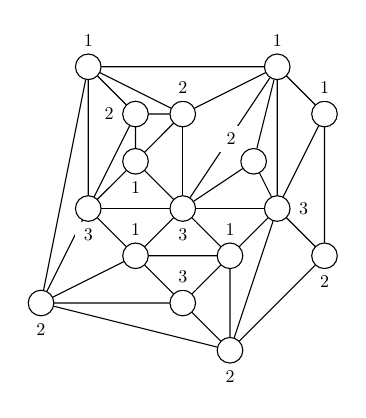
\begin{tikzpicture}[scale=1.2]
    \node (v1) [label=above:${1}$] at (-1cm, 1.5cm) {};
    \node (v2) [label=above:${1}$] at (1cm, 1.5cm) {};
    \node (v3) [label=above:${1}$] at (1.5cm, 1.0cm) {};
    \node (v4) [label=below:${2}$] at (1.5cm, -0.5cm) {};
    \node (v5) [label=below:${2}$] at (0.5cm, -1.5cm) {};
    \node (v6) [label=below:${2}$] at (-1.5cm, -1.0cm) {};

    \node (u1) [label=below:${3}$] at (-1cm, 0.0cm) {};
    \node (u2) [label=below:${3}$] at (0.0cm, 0.0cm) {};
    \node (u3) [label=right:${3}$] at (1cm, 0.0cm) {};

    \node (p1) [label=left:${2}$] at (-0.5cm, 1.0cm) {};
    \node (p2) [label=above:${2}$] at (0.0cm, 1.0cm) {};
    \node (p3) [label=below:${1}$] at (-0.5cm, 0.5cm) {};
    \node (p4) [label=above left:${2}$] at (0.75cm, 0.5cm) {};

    \node (q1) [label=above:${1}$] at (-0.5cm, -0.5cm) {};
    \node (q2) [label=above:${1}$] at (0.5cm, -0.5cm) {};
    \node (q3) [label=above:${3}$] at (0.0cm, -1.0cm) {};

    \begin{pgfonlayer}{bg}
        \draw (v1) edge (v2);
        \draw (v2) edge (v3);
        \draw (v3) edge (v4);
        \draw (v4) edge (v5);
        \draw (v5) edge (v6);
        \draw (v6) edge (v1);

        \draw (v1) edge (u1);
        \draw (v6) edge (u1);
        \draw (v2) edge (u2);
        \draw (v2) edge (u3);
        \draw (v3) edge (u3);
        \draw (v4) edge (u3);
        \draw (v5) edge (u3);

        \draw (v1) edge (p1);
        \draw (v1) edge (p2);
        \draw (v2) edge (p2);
        \draw (v2) edge (p4);

        \draw (v5) edge (q3);
        \draw (v5) edge (q2);
        \draw (v6) edge (q1);
        \draw (v6) edge (q3);

        \draw (u1) edge (p1);
        \draw (u1) edge (p3);
        \draw (u2) edge (p2);
        \draw (u2) edge (p3);
        \draw (u2) edge (p4);
        \draw (u3) edge (p4);

        \draw (u1) edge (q1);
        \draw (u2) edge (q1);
        \draw (u2) edge (q2);
        \draw (u3) edge (q2);

        \draw (u1) edge (u2);
        \draw (u2) edge (u3);

        \draw (p1) edge (p2);
        \draw (p1) edge (p3);
        \draw (p2) edge (p3);

        \draw (q1) edge (q2);
        \draw (q1) edge (q3);
        \draw (q2) edge (q3);
    \end{pgfonlayer}
\end{tikzpicture}
\caption{Algorithm 3.3 example, vertices labelled with $S[v],c[v]$.}
\end{center}
\end{figure}

\begin{algorithm}\label{A:poh_linear}
\textbf{Input:} Assume that $C=v_1,v_2,\ldots,v_k$ is an induced cycle in a weakly
triangulated plane
    graph $G$ with adjacency list representation $\text{Adj}$.

Let $c$ be an array of colors
representing a $2$-coloring of $C$ such
that each color class induces a path, respectively $P_1=v_1,v_2,\ldots,v_i$ and
$P_2=v_{i+1},v_{i+2},\ldots,v_k$. Let $c_{P_1}$ and $c_{P_2}$ be the colors
used on $P_1$ and $P_2$, respectively. Assume that $c[v]=0$ for all
$v\in\text{Int}(C)-C$.

The vertex $v_1$ and the
entry for the edge $v_1v_k$ in $\text{Adj}[v_1]$, together with the
coloring $c$, serve as a representation of $C$, $P_1$, and $P_2$.

Finally, let $S$ be an array of integer marks and let $m_{P_1}$ be an integer
such that for each $v\in\text{Int}(C)-C$ we have $S[v]=m_{P_1}$ if and only if
$v\in N(P_1)$.

\textbf{Output:} Each vertex $v\in\text{Int}(C)-C$, a nonzero color will be
assigned to $c[v]$ such that $c$ represents a path $3$-coloring of
$\text{Int}(C)$ extending the original $2$-coloring of $C$.

\textbf{Step 1:} Let $u$ be the neighbor of $v_1$ immediately clockwise from
$v_k$. If $c[u]\ne 0$ then $u\in C$. But $C$ is an induced cycle, so
it must be that $u=v_2$ and $\text{Int}(C)=C=v_1,v_2,v_3$ with $k=3$ and
$\text{Int}(C)$ is already colored. From now on we will assume that $c[u]=0$ and
$u\not\in C$.

\textbf{Step 2:} Let us color an induced path $P_3$ in $\text{Int}(C)-C$ with the
color $c_{P_3}$ distinct
from the two colors used on
$P_1$ and $P_2$. The new path will start at $u$ and end at the unique verterx
$w\in\text{Int}(C)-C$ such that $w,v_i,v_{i+1}$ is a face. Note that the vertex $w$ is
guaranteed to exist, but in practice we will not a priori
know $w$ before constructing the path $P_3$.

To start, color the vertex $u$ by assigning $c[u]\leftarrow c_{P_3}$. We will
now describe the procedure to color and add a vertex to $P_3$.

Suppose
that we have colored an induced path
$P_3=u_1,u_2,\ldots,u_j$ such that $u_1=u$ and $S[u_\ell]=m_{P_1}$ for each
$\ell\in\{1,2,\ldots,j\}$. Moreover, for each $\ell<j$ assume that no neighbor $y$ of $u_\ell$
between $u_{\ell-1}$ and $u_{\ell +1}$ counter-clocwise satisfies
$S[y]=m_{P_1}$ (consider $u_0=v_k$). Iterate through the neighbors of $u_j$ starting from $u_{j-1}$ until
encountering a neighbor $y$ with $S[y]=m_{P_1}$ or $c[y]=c_{P_1}$.

If $c[y]=c_{P_1}$ then we claim that $y=v_i$ and $u_j=w$. Note that the
neighbor $x$ of $u_j$ immediately clockwise from $y$ is a neighbor of $y$
and therefore satisfies either $c[x]\ne 0$ or $S[x]=m_{P_1}$. But we know
that $c[x]\ne c_{P_1}$ and $S[x]\ne m_{P_1}$, so it must be that
$c[x]=c_{P_2}$. Since $C$ is an induced cycle and $y\in P_1$, $x\in P_2$, it
must be that $y=v_i$ and $x=v_{i+1}$.

If $S[y]=m_{P_1}$, then we claim that $y$ has not already been added to
$P_3$ and that $u_1,u_2,\ldots,u_j,y$ is an induced
path. Since $u_j\in N(P)$ there exists $r\in\{1,2,\ldots,i\}$ such that
$u_jv_r$ is an edge of $\text{Int}(C)$. Note that
$D=v_1,v_2,\ldots,v_r,u_j,u_{j-1},\ldots,u_1$ is a cycle in $\text{Int}(C)$
and $y\not\in\text{Int}(D)$.
Thus if an edge $yu_\ell$ were to exist, it would have to
be between $u_{\ell-1}$ and $u_{\ell+1}$ counter-clockwise in
$\text{Adj}[u_\ell]$, a contradiction
unless $\ell=j$. Therefore we may assign $u_{j+1}\leftarrow y$, color
$c[y]=c_{P_3}$, and continue coloring the path $P_3$.

\textbf{Step 3:} So far we have colored an induced path
$P_3=u_1,u_2,\ldots,u_j$ such that
$C_1=v_1,v_2,\ldots,v_i,u_j,u_{j-1},\ldots,u_1$ and
$C_2=u_1,u_2,\ldots,u_j,v_{i+1},v_{i+2},\ldots,v_k$ are cycles. It remains
to break each cycle down into induced cycles that we may recursively
apply the algorithm to.

To path $3$-color $\text{Int}(C_2)$ let us iterate through the vertices of
$P_3$ starting from $u_1$.
We will keep track of an edge $u_rv_s$ by storing $u_r$ and the entry
for $v_s$ in
$\text{Adj}[u_r]$. Initialize $u_r = u_1$ and $v_s=v_k$. Additinally,
pick $m_{P_3}$ to be a new unique integer mark to identify vertices in
$N(P_3)$.

Let $u_\ell$ be the current vertex and let $u_rv_s$ be the last edge
between $P_3$ and $P_2$ that we have encounterd. Iterate through the neighbors of $u_\ell$
starting from $u_{\ell-1}$ ($v_k$ when $\ell=1$) and stopping at $u_{\ell+1}$
($v_{i+1}$ when $\ell=j$). For each neighbor $y$ of $u_\ell$ we assign
$S[y]=m_{P_3}$. Each time we encounter a neighbor $y$ with
$c[y]=c_{P_2}$, then we know that $y=v_t\in P_2$ and
$C_{r,\ell,s,t}=u_r,u_{r+1},\ldots,u_\ell,v_t,v_{t+1},\ldots,v_t$ is an induced cycle. We
have also marked all vertices in $\text{Int}(C_{r,\ell,s,t})$ in $N(P_3)$
with the unique mark $m_{P_3}$. Make a recursive call to path $3$-color
$\text{Int}(C_{r,\ell,s,t})$ and assign $u_rv_s\leftarrow u_\ell v_t$.

To path $3$-color $\text{Int}(C_1)$ we can follow the same procedure we used
to color $\text{Int}(C_2)$, but instead iterate through $P_3$ backwards from
$u_j$. At each
vertex $u_\ell\in P_3$ we will iterate through the neighbors in
counter-clockwise order from $u_{\ell+1}$ up to $u_{\ell - 1}$.

%\textbf{Step 1:} If $N(P_1)=\emptyset$, then $G-C$ is empty and thus $G$ is
%already path $3$-colored.
%    
%Suppose that $N(P_1)\ne\emptyset$. Let $u,w$ be the vertices in $N(P_1)$ such that $v_1, v_k, u$
%and $v_l,v_{l+1}, w$ are faces of $G$. We will construct
%an induced path $P_3=u_1,\ldots,u_r$ such that $u_1=u$, $u_r=w$, and $u_1,\ldots,u_r\in
%N(P_1)$. Concurrently, we will
%mark all vertices interior to the cycle $C_2=P_3\cup P_2\cup\{v_ku,v_{l+1}w\}$
%with neighbors in $P_3$ and record all
%edges between vertices in $P_3$ and vertices in $P_1$ or $P_2$.
%
%Initialize $u_1=u$. We will also define $u_0$ to be $v_k$ so that
%$u_{i-1}$ is defined when $i=1$.
%
%Let $u_1,\ldots,u_i$ be the the induced path constructed so far. Iterate
%through $\text{Adj}[u_i]$ clockwise starting from $u_{i-1}$ until we reach a
%vertex $u_{i+1}\in N(P_1)$ distinct from $u_{i-1}$ or we reach a vertex in $P_1$. If
%we reach a vertex in $P_1$ first then $u_i$ must be $w$ or there wouldn't exist
%a
%$u,w$-path in $G$ consisting of vertices in $N(P_1)$. If we reach a
%vertex $u_{i+1}\in N(P_1)$ we add it to the path and continue.
%    
%While iterating
%through $\text{Adj}[u_i]$ let us also mark all neighbors between $u_{i-1}$ and
%$u_{i+1}$ to indicate which vertices interior to $C_2$ have neighbors in $P_3$.
%We also record all edges between $u_i$ and vertices in $P_1$ and $P_2$.
%
%\textbf{Step 2:} Color the vertices on the path $P_3$ with the
%remaining color not used on vertices in $P_1$ or $P_2$. Define the cycles
%$C_1=P_1\cup P_3\cup\{v_1u,v_lw\}$ and $C_2=P_3\cup
%P_2\cup\{v_ku,v_{l+1}w\}$. In step 1 we recorded all chords of $C_1$ and
%$C_2$, and also marked all vertices interior to $C_2$ that are in $N(P_3)$.
%Moreover, the vertex marking from the input distinguishes those
%interior to $C_1$ that are in $N(P_1)$; in fact all vertices interior to $C_1$ will be in
%$N(P_1)$. 
%Therefore we may decompose $C_1,C_2$ into induced cycles and apply
%Algorithm~\ref{A:poh_linear} to each.
\end{algorithm}

Note that while executing Algorithm~\ref{A:poh_linear} we only iterate through
the adjacency list of a vertex when it is colored and added
to a path. Therefore the algorithm is linear in the number of vertices.

\section{Path List Coloring: the Hartman-\v{S}krekovski Algorithm}

In this section we will discuss a linear time algorithm for path coloring
plane graphs such that each vertex receives a color from a specified list.
Hartman showed that this is always possible when each vertex is given a
list of $3$ colors~\cite[Thm.~4.1]{Har1997}. Around the same
time \v{S}krekovski proved a
slightly weaker result using the same coloring
strategy~\cite[Thm.~2.2b]{Skr1999}.

The path list-coloring procedure discussed in this section is
based on the constructive proofs found in Hartman and
\v{S}krekovski's papers, but it ``localizes'' the logic to proceed through the
graph one vertex and edge at a time. The resulting algorithm is
similar, but will produce different colorings in some situations.

Let $C$ be the outer face of a weakly triangulated plane graph $G$ and let
$u,v\in C$ be vertices.
If $n(G)\ge3$, then $C$ is a cycle and we
define $C(u,v)$ to be the clockwise path
from $u$ to $v$ around $C$. If $n(G)<3$ then we define $C(u,v)=C$ if
$u\ne v$, and $C(u,u)=u$.

\begin{figure}[h]
\begin{center}
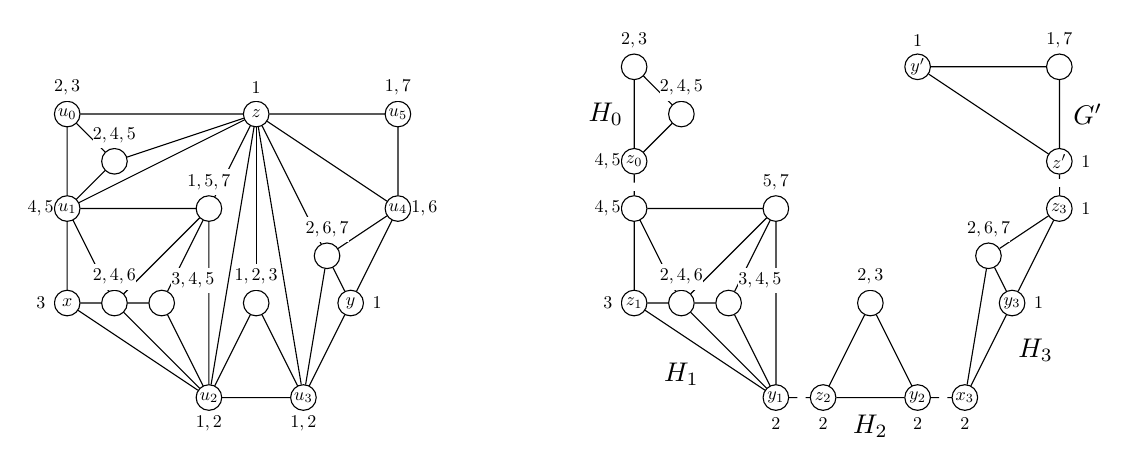
\begin{tikzpicture}[scale=1.2]
    \node (z) [label=above:$1$] at (0.0cm, 1.5cm) {$z$};
    \node (u0) [label=above:${2,3}$] at (-2.0cm, 1.5cm) {$u_0$};
    \node (v0) [label=above:${2,4,5}$] at (-1.5cm, 1.0cm) {};
    \node (u1) [label=left:${4,5}$] at (-2.0cm, 0.5cm) {$u_1$};
    \node (v1) [label=above:${1,5,7}$] at (-0.5cm, 0.5cm) {};
    \node (v2) [label=left:$3$] at (-2.0cm, -0.5cm) {$x$};
    \node (v3) [label=above:${2,4,6}$] at (-1.5cm, -0.5cm) {};
    \node (v4) [label=above right:${3,4,5}$] at (-1.0cm, -0.5cm) {};
    \node (u2) [label=below:${1,2}$] at (-0.5cm, -1.5cm) {$u_2$};
    \node (v5) [label=above:${1,2,3}$] at (0.0cm, -0.5cm) {};
    \node (u3) [label=below:${1,2}$] at (0.5cm, -1.5cm) {$u_3$};
    \node (v6) [label=right:$1$] at (1.0cm, -0.5cm) {$y$};
    \node (v7) [label=above:${2,6,7}$] at (0.75cm, 0.0cm) {};
    \node (u4) [label=right:${1,6}$] at (1.5cm, 0.5cm) {$u_4$};
    \node (u5) [label=above:${1,7}$] at (1.5cm, 1.5cm) {$u_5$};

    \begin{pgfonlayer}{bg} 
        \draw (z) edge (u0);
        \draw (z) edge (u1);
        \draw (z) edge (u2);
        \draw (z) edge (u3);
        \draw (z) edge (u4);
        \draw (z) edge (u5);

        \draw (z) edge (v0);
        \draw (z) edge (v1);
        \draw (z) edge (v5);
        \draw (z) edge (v7);

        \draw (u0) edge (u1);
        \draw (u1) edge (v2);
        \draw (v2) edge (u2);
        \draw (u2) edge (u3);
        \draw (u3) edge (v6);
        \draw (v6) edge (u4);
        \draw (u4) edge (u5);

        \draw (u0) edge (v0);
        \draw (u1) edge (v0);
        \draw (u1) edge (v1);
        \draw (u1) edge (v3);
        \draw (u2) edge (v3);
        \draw (u2) edge (v4);
        \draw (u2) edge (v1);
        \draw (u2) edge (v5);
        \draw (u3) edge (v5);
        \draw (u3) edge (v7);
        \draw (u4) edge (v7);

        \draw (v1) edge (v3);
        \draw (v1) edge (v4);
        \draw (v2) edge (v3);
        \draw (v3) edge (v4);
        \draw (v6) edge (v7);
    \end{pgfonlayer}

    \node (H0) [draw=none, scale=1.5] at (3.7cm, 1.5cm) {$H_0$};
    \node (u0a) [label=above:${2,3}$] at (4.0cm, 2.0cm) {};
    \node (v0a) [label=above:${2,4,5}$] at (4.5cm, 1.5cm) {};
    \node (u1a) [label=left:${4,5}$] at (4.0cm, 1.0cm) {$z_0$};

    \node (H1) [draw=none, scale=1.5] at (4.5cm, -1.25cm) {$H_1$};
    \node (u1b) [label=left:${4,5}$] at (4.0cm, 0.5cm) {};
    \node (v1b) [label=above:${5,7}$] at (5.5cm, 0.5cm) {};
    \node (v2b) [label=left:$3$] at (4.0cm, -0.5cm) {$z_1$};
    \node (v3b) [label=above:${2,4,6}$] at (4.5cm, -0.5cm) {};
    \node (v4b) [label=above right:${3,4,5}$] at (5.0cm, -0.5cm) {};
    \node (u2b) [label=below:$2$] at (5.5cm, -1.5cm) {$y_1$};

    \node (H2) [draw=none, scale=1.5] at (6.5cm, -1.8cm) {$H_2$};
    \node (u2c) [label=below:$2$] at (6.0cm, -1.5cm) {$z_2$}; 
    \node (v5c) [label=above:${2,3}$] at (6.5cm, -0.5cm) {};
    \node (u3c) [label=below:$2$] at (7.0cm, -1.5cm) {$y_2$};

    \node (H3) [draw=none, scale=1.5] at (8.25cm, -1.0cm) {$H_3$};
    \node (u3d) [label=below:$2$] at (7.5cm, -1.5cm) {$x_3$};
    \node (v6d) [label=right:$1$] at (8.0cm, -0.5cm) {$y_3$};
    \node (v7d) [label=above:${2,6,7}$] at (7.75cm, 0.0cm) {};
    \node (u4d) [label=right:$1$] at (8.5cm, 0.5cm) {$z_3$};

    \node (H4) [draw=none, scale=1.5] at (8.8cm, 1.5cm) {$G'$};
    \node (u4e) [label=right:$1$] at (8.5cm, 1.0cm) {$z'$};
    \node (u5e) [label=above:${1,7}$] at (8.5cm, 2.0cm) {};
    \node (ze) [label=above:$1$] at (7.0cm, 2.0cm) {$y'$};

    \begin{pgfonlayer}{bg}
        \draw (u0a) edge (u1a);
        \draw (u0a) edge (v0a);
        \draw (u1a) edge (v0a);

        \draw (u1a) edge [dashed] (u1b);

        \draw (u1b) edge (v2b);
        \draw (v2b) edge (u2b);
        \draw (u1b) edge (v1b);
        \draw (u1b) edge (v3b);
        \draw (u2b) edge (v3b);
        \draw (u2b) edge (v4b);
        \draw (u2b) edge (v1b);
        \draw (v1b) edge (v3b);
        \draw (v1b) edge (v4b);
        \draw (v2b) edge (v3b);
        \draw (v3b) edge (v4b);

        \draw (u2b) edge [dashed] (u2c);

        \draw (u2c) edge (u3c);
        \draw (u2c) edge (v5c);
        \draw (u3c) edge (v5c);

        \draw (u3c) edge [dashed] (u3d);

        \draw (u3d) edge (v6d);
        \draw (v6d) edge (u4d);
        \draw (v6d) edge (v7d);
        \draw (u3d) edge (v7d);
        \draw (u4d) edge (v7d);

        \draw (u4d) edge [dashed] (u4e);

        \draw (ze) edge (u4e);
        \draw (ze) edge (u5e);
        \draw (u4e) edge (u5e);
    \end{pgfonlayer}
\end{tikzpicture}
\caption{A step of Algorithm~\ref{A:hartman3} (if $z_\ell=x_\ell$
and/or $z_\ell=y_\ell$, only $z_\ell$ is labelled).}
\end{center}
\end{figure}

\begin{algorithm}[Hartman 1997, \v{S}krekovski 1999]\label{A:hartman3}
\textbf{Input:} Let $G$ be a weakly triangulated plane graph with outer face
$C$. Let $x,y,z\in C$ be vertices (not necessarily distinct) such that
$z\in C(x,y)$. Finally, let $L:V(G)\to P_{<\aleph_0}(\mathbb{N})$ be a
function assigning a finite list of colors to
each vertex such that
\begin{align*}
    |L(v)| &\ge 1 \text{ for } v\in\{x,y,z\} \\
    |L(v)| &\ge 2 \text{ for } v\in C-\{x,y,z\} \\
    |L(v)| &\ge 3 \text{ for } v\in G-C,
\end{align*}
    and if $u\in C(x,z)-z$, then $L(u)\cap L(z)=\emptyset$.

\textbf{Output:} A path $3$-coloring $c:V(G)\to\mathbb{N}$ of $G$ such
    that $c(v)\in L(v)$ for all $v\in G$ and $\text{deg}_c(x)\le 1$,
    $\text{deg}_c(y)\le 1$, and $\text{deg}_c(z)\le 1$. Furthermore, if
    $v\in G-C(z,y)$ is a neighbor of $z$, then $c(z)\ne c(v)$.
 
    \textbf{Step 1:} For each $v\in\{x,y,z\}$ assign
    $c(v)$ to be a color in $L(v)$. If $x,y,z$ are the only vertices in
    $G$, then we are done. If $n(G)=2$ and $x=y=z$, then the remaining
    vertex $v\in G-x$ satisfies $|L(v)-c(z)|\ge2$
    and we may choose $c(v)$ to be an arbitrary color in $L(v)-c(z)$.
    From now on assume that $n(G)>2$ and the outer
    face $C$ is a cycle.

    \textbf{Step 2:}
    We will recursively apply the algorithm to path $L$-choose
    the $2$-connected components of $G-z$. Note that each cut-vertex of $G-z$
    must be a neighbor of $z$ in $C$. Therefore each cut-vertex will
    exist in at most
    two $2$-connected components and the ``graph of $2$-connected
    components'' of $G-z$ is a path. Let us label these
    $2$-connected components $H_1,H_2,\ldots,H_{k-1}$ in counter-clockwise
    order from $z$ around $C$. Let us similarly label the neighbors
    of $z$ in counter-clockwise order as $u_1,\ldots,u_{k}$. Note that
    the neighgors $u_2,\ldots,u_{k-1}$ are the cut-vertices of $G-z$ and each
    $u_\ell$ is contained in $H_{\ell-1}$ and $H_{\ell}$.

    Suppose that $u_1=y$. Then since $z\in C(x,y)$, it must be that $x=z$.
    We may re-label $x'=y$, $z'=y$, $y'=z$ and apply the algorithm to path
    $L$-choose $G$ with the same color degree guarantees on $x$, $y$, and
    $z$. Thus we may assume that $u_1\ne y$. 

    If $z\ne x$ then let $H_i$ be the $2$-connected
    component containing $x$; if $x=u_i$ is a cut-vertex, and is therfore
    contained two components $H_i$ and $H_{i+1}$, we
    single out the component $H_i$.
    If $z=x$, define $i=1$.

    Similarly, if $z\ne y$ define $H_j$ to be the
    component containing $y$; if $y=u_{j+1}$ is a cut-vertex, then pick
    the component $H_j$ ($j>0$ since $u_1\ne y$).
    If $z = y$ then define $j=k$.
    Observe that $1\le i\le j\le k$.

    For any $a,b\in\{1,2,\ldots,k\}$ such that $a\le b$ define

    $$ G_{a,b}=G\left[\{z\}\cup V(H_a)\cup V(H_{a+1})\cup \ldots\cup V(H_b)\right].$$ 

    We will $L$-choose the $2$-connected components of $G-z$ in the order

    $$H_i,H_{i+1},\ldots,H_j,H_{i-1},H_{i-2},\ldots,H_1$$

    to produce a path $L$-choosing of $G_{1,j}$. Finally,
    if $j < k$, we will
    path $L$-choose $G_{j+1,k}$ as a separate case.

    \textbf{Step 2.1:} To start we will path $L$-choose $G_{i,i}$.

    \textbf{Case 2.1.1:} Suppose that $i=j$ and therefore
    $G_{i,i}=G_{i,j}$. 

    If $c(z)\in L(u_{i+1})$ then define
    $L_i(u_{i+1})=\{c(z)\}$ and $L(v)=L(v)\setminus\{c(z)\}$ for
    $v\in H_i-u_{i+1}$. Recursively path $L_i$-choose $H_i$ with $x_i=x$, $y_i=y$,
    and $z_i=u_{i+1}$. The $L_i$-choosing of $H_i$ extends to a path
    $L$-choosing of $G_{i,j}$ such that $\text{deg}_c(x)\le 1$,
    $\text{deg}_c(y)\le 1$, and $\text{deg}_c(z)=1$.

    Otherwise, $c(z)\not\in L(u_{i+1})$. Define $L_i(v)=L(v)\setminus\{c(z)\}$
    for all $v\in H_i$ and note that $|L_i(u_{i+1})|\ge 2$. Path
    $L_i$-choose $H_i$ with $x_i=x$, $y_i=y$, and $z_i=x$. This $L_i$-choosing
    extends to a path $L$-choosing of $G_{i,j}$ with
    $\text{deg}_c(x)\le 1$, $\text{deg}_c(y)\le 1$, and $\text{deg}_c(z)=0$.

    \textbf{Case 2.1.2:} Suppose that $i\ne j$.
    Define $L_i(v)=L(v)\setminus\{c(z)\}$ for all $v\in H_i$. Recall that
    $u_i\in C(x,z)-z$, thus $L(u_i)\cap L(z)=\emptyset$ and $L_i(u_i)=L(u_i)$. 

    If $z=x$ or if $x=u_i$ is a cut-vertex, then we
    define $x_i=u_i$, $z_i=u_i$, and $y_i=u_{i+1}$ and apply the algorithm
    to path $L_i$-choose $H_i$. Note that if $z=x$ then $i=1$ and $x_1=u_1$
    is the vertex immediately counter-clockwise to $z$ around $C$.

    Otherwise $x$ is not a cut-vertex. Note that $u_i\in C(x,z) - z$ and
    therefore $|L'(u_i)|\ge 2$. Thus we may define $x_i=x$, $z_i=x$,
    $y_i=u_{i+1}$ and path $L_i$-choose $H_i$.

    In both cases the path $L_i$-choosing of $H_i$ extends to a path
    $L$-choosing of $G_{i,i}$ such that $\text{deg}_c(u_{i+1})\le 1$,
    $\text{deg}_c(x)\le 1$, and $\text{deg}_c(z)=0$. 

    \textbf{Step 2.2:} Suppose that $\ell\in\{i+1, i+2,\ldots,j-1\}$
    and we have computed a path $L$-choosing of $G_{i,\ell-1}$ such that
    $\text{deg}_c(u_\ell)\le1$, $\text{deg}_c(x)\le 1$,
    and $\text{deg}_c(z)=0$.

    Define $L_\ell(u_\ell)=\{c(u_\ell)\}$ and
    $L_\ell(v)=L(v)\setminus\{c(z)\}$ for
    all $v\in H_\ell-u_\ell$.
    Path $L_\ell$-choose $H_\ell$ with
    $x_\ell=u_\ell$, $z_\ell=u_\ell$, and
    $y_\ell=u_{\ell+1}$. We are guaranteed that the path $L$-choosing
    of $G_{i,\ell-1}$ and the path $L_\ell$-choosing of $H_\ell$ agree
    at the shared vertex $u_\ell$, and that
    $\text{deg}_c(u_\ell)\le 1$ and $\text{deg}_c(u_{\ell+1})\le 1$
    in $H_\ell$. Taken together they form a
    path $L$-list coloring of $G_{i,\ell}$ with $\text{deg}_c(u_{\ell+1})\le 1$,
    $\text{deg}_c(x)\le 1$, and $\text{deg}_c(z)=0$.

    \textbf{Step 2.3:} Suppose that $i\ne j$ and we
    have computed a path $L$-list-colroing of $G_{i,j-1}$ such that
    $\text{deg}_c(u_j)=1$, $\text{deg}_c(x)\le 1$, and $\text{deg}_c(z)=0$. 

    If $z=y$, then
    define $x_j=u_j$, $z_j=u_j$, $y_j=u_{j+1}$, and
    $L_j(v)=L(v)\setminus\{c(z)\}$ for all $v\in H_j$. Path $L_j$-choose
    $H_j$ and note that it extends to form a path
    $L$-choosing of $G_{i,j}$ with
    $\text{deg}_c(z)=0$ via the same argument from Step 2.2.

    Otherwise $z\ne y$ and $u_{j+1}$ is the furthest clockwise neighbor of $z$
    around $C$ in $C(z,y)$. If $c(z)\in L(u_{j+1})$, then define
    $L_j(u_{j+1})=\{c(z)\}$ and $L_j(v)=L(v)\setminus\{c(z)\}$ for all $v\in
    H_j-u_{j+1}$. Path $L_j$-choose $H_j$ with $x_j=u_j$,
    $z_j=u_{j+1}$, and $y_j=y$. Again the path $L_j$-choosing of $H_j$
    agrees with the path $L$-choosing
    of $G_{i,j-1}$ and both combine to a path $L$-choosing
    of $G_{i,j}$ such that $\text{deg}_c(z)=1$.

    If $c(z)\not\in L(u_{j+1})$
    then define $L_j(v)=L(v)\setminus\{c(z\}$ for all $v\in H_j$. Note that
    $|L_j(u_{j+1})|\ge 2$, thus we may path $L_j$-choose $H_j$ with
    $x_j=u_j$, $z_j=u_j$, and $y_j=y$. The $L_j$-choosing extends to path
    $L$-choosing of $G_{i,j}$ with $\text{deg}_c(z)=0$.

    \textbf{Step 2.4:} We will
    now color any remaining components $H_\ell$ with
    $\ell<i$. Suppose that $\ell\in \{1,2,..,i-1\}$ and that we have
    computed a path
    $L$-choosing of $G_{\ell+1,j}$ such that $\text{deg}_c(z)\le 1$. Define
    $L_\ell(u_{\ell+1})=\{c(u_{\ell+1})\}$
    and $L_\ell(v)=L(v)\setminus\{c(z)\}$
    for all $v\in H_\ell-u_\{\ell+1\}$. Path $L_\ell$-choose $H_\ell$ with
    $x_\ell=u_{\ell+1}$, $y_\ell=u_{\ell+1}$, and $z_\ell=u_{\ell+1}$.
    Note that $\text{deg}_c(u_{\ell+1})=0$ in $H_\ell$ and therefore the
    $L_\ell$-choosing
    extends to a path $L$-choosing of $G_{\ell,j}$ with $\text{deg}_c(z)\le
    1$.

    \textbf{Step 2.5:} If $j=k$, then the above steps have computed a path
    $L$-choosing of $G$. Otherwise it remains to extend the $L$-choosing
    to $G_{j+1,k}$.

    Define $L'(u_{j+1})=\{c(u_{j+1})\}$, $L'(z)=\{c(z)\}$, and $L'(v)=L(v)$ for
    $v\in G_{j+1,k}-\{u_{j+1},z\}$. We
    then path $L'$-choose $G'=G_{j+1,k}$ with $x'=u_{j+1}$,
    $z'=u_{j+1}$, and $y'=z$.
    Taking $C'$ to be the outer face of $G'$ note that
    $C'(x',y')$ is the two vertex path $x',y'$. Therefore no neighbor of $x'$
    other than $y'$ will be assigned the color $c(x')$.

    By Step 2.4, either $\text{deg}_c(z)=0$ in $G_{1,j}$ or
    $c(u_{j+1})=c(z)$ and $\text{deg}_c(z)=1$.
    Because
    $$V(G_{1,j})\cap V(G_{j+1,k})=\{z,u_{j+1}\}=\{x',y'\},$$
    the path
    $L$-choosing of $G_{1,j}$ and the path $L'$-choosing of $G_{j+1,k}$
    agree and extend to a path $L$-choosing of $G$ such that
    $\text{deg}_c(x)\le1$,
    $\text{deg}_c(y)\le 1$, and $\text{deg}_c(z)\le 1$.
\end{algorithm}

%\begin{tikzpicture}
%  \node (u0) [label=above left:$u_0$, fill] at (-1.28cm, 1.8cm) {};
%  \node (z) [label=above:{$z$}] at (0cm, 2cm) {};
%  \node (u7) [label=above right:$u_k$] at (1.28cm, 1.8cm) {};
%  \node (u1) [label=left:$u_1$, fill] at (-1.97cm, 0.35cm) {};
%  \node (u2) [label=below left:$u_i$] at (-1.73cm, -1.0cm) {};
%    \node (u3) [label=below:$u_{i+1}$] at (-0.68cm, -1.88cm) {};
%  \node (u4) [label=below:$u_j$] at (0.68cm, -1.88cm) {};
%    \node (u5) [label=below right:$u_{j+1}$] at (1.73cm, -1.0cm) {};
%    \node (u6) [label=right:$u_{k-1}$] at (1.96cm, 0.34cm) {};
%  \node (x) [label=below left:$x$] at (-1.29cm, -1.53cm) {};
%  \node (y) [label=below right:$y$] at (1.29cm, -1.53cm) {};
% 
%  \draw (z) edge (u7);
%  \draw (u7) edge (u6) [dashed];
%  \draw (u6) edge (u5) [dashed];
%  \draw (u5) edge (y) [dashed];
%  \draw (y) edge (u4) [dashed];
%  \draw (u4) edge (u3) [dashed];
%  \draw (u3) edge (x) [dashed];
%  \draw (x) edge (u2) [dashed];
%  \draw (u2) edge (u1) [dashed];
%  \draw (u1) edge (u0) [dashed];
%  \draw (u0) edge (z);
%
%  \draw (u7) to[out=190, in=130] (u6) [dashed];
%  \draw (u6) to[out=155, in=115] (u5) [dashed];
%  \draw (u5) to[out=125, in=95] (u4) [dashed];
%  \draw (u4) edge [bend right=75] (u3) [dashed];
%  \draw (u3) to[out=85, in=55] (u2) [dashed];
%  \draw (u2) to[out=65, in=25] (u1) [dashed];
%  \draw (u1) to[out=50, in=350] (u0) [dashed];
%
%  \draw (z) edge (u1);
%  \draw (z) edge (u2);
%  \draw (z) edge (u3);
%  \draw (z) edge (u4);
%  \draw (z) edge (u5);
%  \draw (z) edge (u6);
%\end{tikzpicture}

Algorithm~\ref{A:hartman3} may be implemented for plane graphs represented by
rotation scheme ordered augmented adjacency lists in $\mathcal{O}(n)$ time.
For each vertex $v\in G$ the implementation will track a list $L[v]$ of up to
three colors,
a integer location mark $S[v]$, and a pair $N[v]=(r_1,r_2)$ of refernces to
neighbor entries in $v$'s augmented adjacency list.

The pair of references to
the adjacency list of $v\in C$
will be the entries for the vertices preceeding and succeeding $v$ clockwise
around $C$. The references provide a representation of $\text{Int}(C)$ and a
quick way to walk around $C$.
 
We can track vertex locations on the outer face by marking each vertex in
$C_\ell(u_\ell,u_{\ell + 1})-u_{\ell+1}$ with a new unique mark.
In Step 2.1 when $z\ne x$ we must instead
mark the vertices in $C_i(u_i,u_{i+1})-u_{i+1}$ with the mark $S[x]$ 
already assigned to the vertices in $C(x,u_i)=C_i(x,u_i)$.

In Step 2.1.1 or Step 2.3 when $z\ne y$ and $c(z)\not\in L(u_{j+1})$,
the segment $C_j(z_j,y)=C_j(x_j,y)$ will consist of vertices in $G-C$
marked with the new mark $S[u_j]$, as well as vertices in $C(u_{j+1},y)$ marked with $S[y]$.
To proceed with the algorithm, we need these two distinct marks to compare
equal and represent the single face segment $C(x_j,y)$.
To accomplish this re-marking efficiently, we
will track a separate array $M$ initialized such that
$M[m]=m$ for each integer mark $m$.
Whenever a mark $S[v]$ is compared with the mark $S[y]$, we will
instead compare
$M[S[v]]$ with $S[y]$. Then to join the segment $C_j(u_j,u_{j+1})$ marked with
$S[u_j]$ and the segment $C_j(u_{j+1},y)$ marked with $S[y]$ we can simply
assign $M[S[u_j]]=S[y]$.

\begin{figure}
\begin{center}
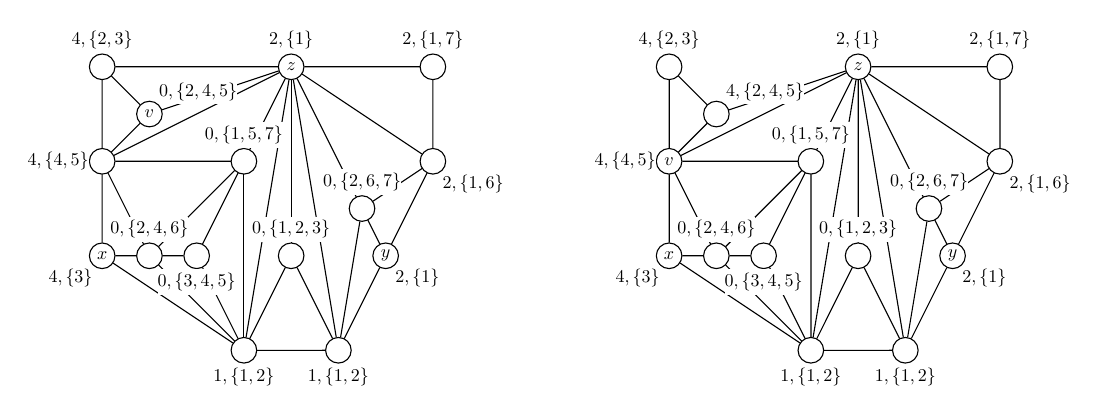
\begin{tikzpicture}[scale=1.2]
    \node (z) [label=above:${2, \{1\}}$] at (0.0cm, 1.5cm) {$z$};
    \node (u0) [label=above:${4,\{2,3\}}$] at (-2.0cm, 1.5cm) {};
    \node (v0) [label=above right:${0,\{2,4,5\}}$] at (-1.5cm, 1.0cm) {$v$};
    \node (u1) [label=left:${4,\{4,5\}}$] at (-2.0cm, 0.5cm) {};
    \node (v1) [label=above:${0,\{1,5,7\}}$] at (-0.5cm, 0.5cm) {};
    \node (v2) [label=below left:${4,\{3\}}$] at (-2.0cm, -0.5cm) {$x$};
    \node (v3) [label=above:${0,\{2,4,6\}}$] at (-1.5cm, -0.5cm) {};
    \node (v4) [label=below:${0,\{3,4,5\}}$] at (-1.0cm, -0.5cm) {};
    \node (u2) [label=below:${1,\{1,2\}}$] at (-0.5cm, -1.5cm) {};
    \node (v5) [label=above:${0,\{1,2,3\}}$] at (0.0cm, -0.5cm) {};
    \node (u3) [label=below:${1,\{1,2\}}$] at (0.5cm, -1.5cm) {};
    \node (v6) [label=below right:${2,\{1\}}$] at (1.0cm, -0.5cm) {$y$};
    \node (v7) [label=above:${0,\{2,6,7\}}$] at (0.75cm, 0.0cm) {};
    \node (u4) [label=below right:${2,\{1,6\}}$] at (1.5cm, 0.5cm) {};
    \node (u5) [label=above:${2,\{1,7\}}$] at (1.5cm, 1.5cm) {};

    \begin{pgfonlayer}{bg} 
        \draw (z) edge (u0);
        \draw (z) edge (u1);
        \draw (z) edge (u2);
        \draw (z) edge (u3);
        \draw (z) edge (u4);
        \draw (z) edge (u5);

        \draw (z) edge (v0);
        \draw (z) edge (v1);
        \draw (z) edge (v5);
        \draw (z) edge (v7);

        \draw (u0) edge (u1);
        \draw (u1) edge (v2);
        \draw (v2) edge (u2);
        \draw (u2) edge (u3);
        \draw (u3) edge (v6);
        \draw (v6) edge (u4);
        \draw (u4) edge (u5);

        \draw (u0) edge (v0);
        \draw (u1) edge (v0);
        \draw (u1) edge (v1);
        \draw (u1) edge (v3);
        \draw (u2) edge (v3);
        \draw (u2) edge (v4);
        \draw (u2) edge (v1);
        \draw (u2) edge (v5);
        \draw (u3) edge (v5);
        \draw (u3) edge (v7);
        \draw (u4) edge (v7);

        \draw (v1) edge (v3);
        \draw (v1) edge (v4);
        \draw (v2) edge (v3);
        \draw (v3) edge (v4);
        \draw (v6) edge (v7);
    \end{pgfonlayer}

    \node (zb) [label=above:${2, \{1\}}$] at (6.0cm, 1.5cm) {$z$};
    \node (u0b) [label=above:${4,\{2,3\}}$] at (4.0cm, 1.5cm) {};
    \node (v0b) [label=above right:${4,\{2,4,5\}}$] at (4.5cm, 1.0cm) {};
    \node (u1b) [label=left:${4,\{4,5\}}$] at (4.0cm, 0.5cm) {$v$};
    \node (v1b) [label=above:${0,\{1,5,7\}}$] at (5.5cm, 0.5cm) {};
    \node (v2b) [label=below left:${4,\{3\}}$] at (4.0cm, -0.5cm) {$x$};
    \node (v3b) [label=above:${0,\{2,4,6\}}$] at (4.5cm, -0.5cm) {};
    \node (v4b) [label=below:${0,\{3,4,5\}}$] at (5.0cm, -0.5cm) {};
    \node (u2b) [label=below:${1,\{1,2\}}$] at (5.5cm, -1.5cm) {};
    \node (v5b) [label=above:${0,\{1,2,3\}}$] at (6.0cm, -0.5cm) {};
    \node (u3b) [label=below:${1,\{1,2\}}$] at (6.5cm, -1.5cm) {};
    \node (v6b) [label=below right:${2,\{1\}}$] at (7.0cm, -0.5cm) {$y$};
    \node (v7b) [label=above:${0,\{2,6,7\}}$] at (6.75cm, 0.0cm) {};
    \node (u4b) [label=below right:${2,\{1,6\}}$] at (7.5cm, 0.5cm) {};
    \node (u5b) [label=above:${2,\{1,7\}}$] at (7.5cm, 1.5cm) {};

    \begin{pgfonlayer}{bg} 
        \draw (zb) edge (u1b);
        \draw (zb) edge (u2b);
        \draw (zb) edge (u3b);
        \draw (zb) edge (u4b);
        \draw (zb) edge (u5b);

        \draw (zb) edge (v0b);
        \draw (zb) edge (v1b);
        \draw (zb) edge (v5b);
        \draw (zb) edge (v7b);

        \draw (u0b) edge (u1b);
        \draw (u1b) edge (v2b);
        \draw (v2b) edge (u2b);
        \draw (u2b) edge (u3b);
        \draw (u3b) edge (v6b);
        \draw (v6b) edge (u4b);
        \draw (u4b) edge (u5b);

        \draw (u0b) edge (v0b);
        \draw (u1b) edge (v0b);
        \draw (u1b) edge (v1b);
        \draw (u1b) edge (v3b);
        \draw (u2b) edge (v3b);
        \draw (u2b) edge (v4b);
        \draw (u2b) edge (v1b);
        \draw (u2b) edge (v5b);
        \draw (u3b) edge (v5b);
        \draw (u3b) edge (v7b);
        \draw (u4b) edge (v7b);

        \draw (v1b) edge (v3b);
        \draw (v1b) edge (v4b);
        \draw (v2b) edge (v3b);
        \draw (v3b) edge (v4b);
        \draw (v6b) edge (v7b);
    \end{pgfonlayer}
\end{tikzpicture}
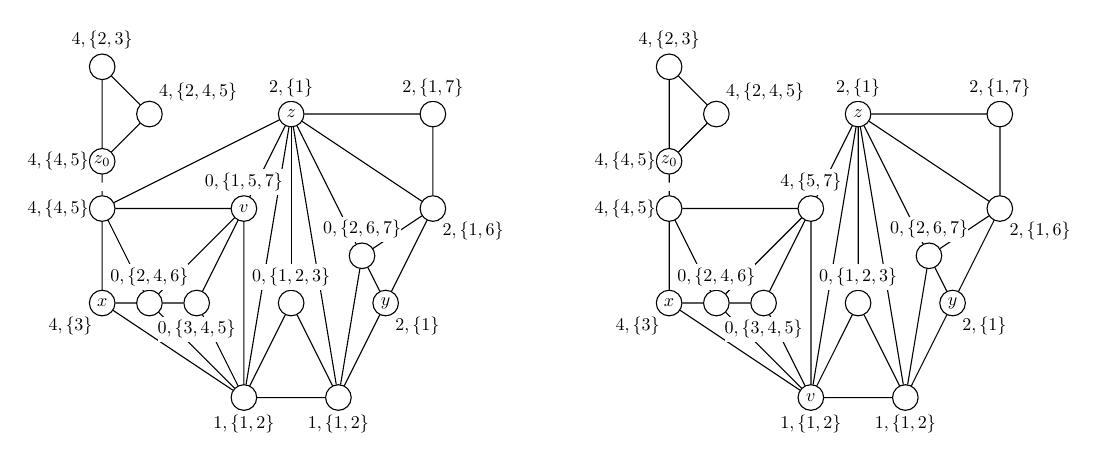
\begin{tikzpicture}[scale=1.2]
    \node (u0r) [label=above:${4,\{2,3\}}$] at (-2.0cm, 2.0cm) {};
    \node (v0r) [label=above right:${4,\{2,4,5\}}$] at (-1.5cm, 1.5cm) {};
    \node (u1r) [label=left:${4,\{4,5\}}$] at (-2.0cm, 1.0cm) {$z_0$};

    \node (z) [label=above:${2, \{1\}}$] at (0.0cm, 1.5cm) {$z$};
    \node (u1) [label=left:${4,\{4,5\}}$] at (-2.0cm, 0.5cm) {};
    \node (v1) [label=above:${0,\{1,5,7\}}$] at (-0.5cm, 0.5cm) {$v$};
    \node (v2) [label=below left:${4,\{3\}}$] at (-2.0cm, -0.5cm) {$x$};
    \node (v3) [label=above:${0,\{2,4,6\}}$] at (-1.5cm, -0.5cm) {};
    \node (v4) [label=below:${0,\{3,4,5\}}$] at (-1.0cm, -0.5cm) {};
    \node (u2) [label=below:${1,\{1,2\}}$] at (-0.5cm, -1.5cm) {};
    \node (v5) [label=above:${0,\{1,2,3\}}$] at (0.0cm, -0.5cm) {};
    \node (u3) [label=below:${1,\{1,2\}}$] at (0.5cm, -1.5cm) {};
    \node (v6) [label=below right:${2,\{1\}}$] at (1.0cm, -0.5cm) {$y$};
    \node (v7) [label=above:${0,\{2,6,7\}}$] at (0.75cm, 0.0cm) {};
    \node (u4) [label=below right:${2,\{1,6\}}$] at (1.5cm, 0.5cm) {};
    \node (u5) [label=above:${2,\{1,7\}}$] at (1.5cm, 1.5cm) {};

    \begin{pgfonlayer}{bg} 
        \draw (u0r) edge (u1r);
        \draw (u0r) edge (v0r);
        \draw (u1r) edge (v0r);

        \draw (u1r) edge [dashed] (u1);

        \draw (z) edge (u1);
        \draw (z) edge (u2);
        \draw (z) edge (u3);
        \draw (z) edge (u4);
        \draw (z) edge (u5);

        \draw (z) edge (v1);
        \draw (z) edge (v5);
        \draw (z) edge (v7);

        \draw (u1) edge (v2);
        \draw (v2) edge (u2);
        \draw (u2) edge (u3);
        \draw (u3) edge (v6);
        \draw (v6) edge (u4);
        \draw (u4) edge (u5);

        \draw (u1) edge (v1);
        \draw (u1) edge (v3);
        \draw (u2) edge (v3);
        \draw (u2) edge (v4);
        \draw (u2) edge (v1);
        \draw (u2) edge (v5);
        \draw (u3) edge (v5);
        \draw (u3) edge (v7);
        \draw (u4) edge (v7);

        \draw (v1) edge (v3);
        \draw (v1) edge (v4);
        \draw (v2) edge (v3);
        \draw (v3) edge (v4);
        \draw (v6) edge (v7);
    \end{pgfonlayer}

    \node (u0br) [label=above:${4,\{2,3\}}$] at (4.0cm, 2.0cm) {};
    \node (v0br) [label=above right:${4,\{2,4,5\}}$] at (4.5cm, 1.5cm) {};
    \node (u1br) [label=left:${4,\{4,5\}}$] at (4.0cm, 1.0cm) {$z_0$};

    \node (zb) [label=above:${2, \{1\}}$] at (6.0cm, 1.5cm) {$z$};
    \node (u1b) [label=left:${4,\{4,5\}}$] at (4.0cm, 0.5cm) {};
    \node (v1b) [label=above:${4,\{5,7\}}$] at (5.5cm, 0.5cm) {};
    \node (v2b) [label=below left:${4,\{3\}}$] at (4.0cm, -0.5cm) {$x$};
    \node (v3b) [label=above:${0,\{2,4,6\}}$] at (4.5cm, -0.5cm) {};
    \node (v4b) [label=below:${0,\{3,4,5\}}$] at (5.0cm, -0.5cm) {};
    \node (u2b) [label=below:${1,\{1,2\}}$] at (5.5cm, -1.5cm) {$v$};
    \node (v5b) [label=above:${0,\{1,2,3\}}$] at (6.0cm, -0.5cm) {};
    \node (u3b) [label=below:${1,\{1,2\}}$] at (6.5cm, -1.5cm) {};
    \node (v6b) [label=below right:${2,\{1\}}$] at (7.0cm, -0.5cm) {$y$};
    \node (v7b) [label=above:${0,\{2,6,7\}}$] at (6.75cm, 0.0cm) {};
    \node (u4b) [label=below right:${2,\{1,6\}}$] at (7.5cm, 0.5cm) {};
    \node (u5b) [label=above:${2,\{1,7\}}$] at (7.5cm, 1.5cm) {};

    \begin{pgfonlayer}{bg} 
        \draw (u0br) edge (v0br);
        \draw (u1br) edge (v0br);
        \draw (u0br) edge (u1br);

        \draw (u1br) edge [dashed] (u1b);

        \draw (zb) edge (u2b);
        \draw (zb) edge (u3b);
        \draw (zb) edge (u4b);
        \draw (zb) edge (u5b);

        \draw (zb) edge (v1b);
        \draw (zb) edge (v5b);
        \draw (zb) edge (v7b);

        \draw (u1b) edge (v2b);
        \draw (v2b) edge (u2b);
        \draw (u2b) edge (u3b);
        \draw (u3b) edge (v6b);
        \draw (v6b) edge (u4b);
        \draw (u4b) edge (u5b);

        \draw (u1b) edge (v1b);
        \draw (u1b) edge (v3b);
        \draw (u2b) edge (v3b);
        \draw (u2b) edge (v4b);
        \draw (u2b) edge (v1b);
        \draw (u2b) edge (v5b);
        \draw (u3b) edge (v5b);
        \draw (u3b) edge (v7b);
        \draw (u4b) edge (v7b);

        \draw (v1b) edge (v3b);
        \draw (v1b) edge (v4b);
        \draw (v2b) edge (v3b);
        \draw (v3b) edge (v4b);
        \draw (v6b) edge (v7b);
    \end{pgfonlayer}
\end{tikzpicture}
\begin{tikzpicture}[scale=1.2]
    \node (u0r) [label=above:${4,\{2,3\}}$] at (-2.0cm, 2.0cm) {};
    \node (v0r) [label=above right:${4,\{2,4,5\}}$] at (-1.5cm, 1.5cm) {};
    \node (u1r) [label=left:${4,\{4,5\}}$] at (-2.0cm, 1.0cm) {$z_0$};

    \node (u1s) [label=left:${4,\{4,5\}}$] at (-2.0cm, 0.5cm) {};
    \node (v1s) [label=above:${4,\{5,7\}}$] at (-0.5cm, 0.5cm) {};
    \node (v2s) [label=below left:${4,\{3\}}$] at (-2.0cm, -0.5cm) {$z_1$};
    \node (v3s) [label=above:${0,\{2,4,6\}}$] at (-1.5cm, -0.5cm) {};
    \node (v4s) [label=below:${0,\{3,4,5\}}$] at (-1.0cm, -0.5cm) {};
    \node (u2s) [label=below left:${4,\{2\}}$] at (-0.5cm, -1.5cm) {$y_1$};

    \node (z) [label=above:${2, \{1\}}$] at (0.5cm, 1.5cm) {$z$};
    \node (u2) [label=below:${5,\{2\}}$] at (0.0cm, -1.5cm) {$x$};
    \node (v5) [label=above:${0,\{1,2,3\}}$] at (0.5cm, -0.5cm) {$v$};
    \node (u3) [label=below:${1,\{1,2\}}$] at (1.0cm, -1.5cm) {};
    \node (v6) [label=below right:${2,\{1\}}$] at (1.5cm, -0.5cm) {$y$};
    \node (v7) [label=above:${0,\{2,6,7\}}$] at (1.25cm, 0.0cm) {};
    \node (u4) [label=below right:${2,\{1,6\}}$] at (2.0cm, 0.5cm) {};
    \node (u5) [label=above:${2,\{1,7\}}$] at (2.0cm, 1.5cm) {};

    \begin{pgfonlayer}{bg} 
        \draw (u0r) edge (u1r);
        \draw (u0r) edge (v0r);
        \draw (u1r) edge (v0r);

        \draw (u1r) edge [dashed] (u1s);

        \draw (u1s) edge (v2s);
        \draw (v2s) edge (u2s);
        \draw (u1s) edge (v1s);
        \draw (u1s) edge (v3s);
        \draw (u2s) edge (v3s);
        \draw (u2s) edge (v4s);
        \draw (u2s) edge (v1s);

        \draw (u2s) edge [dashed] (u2);

        \draw (z) edge (u2);
        \draw (z) edge (u3);
        \draw (z) edge (u4);
        \draw (z) edge (u5);

        \draw (z) edge (v5);
        \draw (z) edge (v7);


        \draw (u2) edge (u3);
        \draw (u3) edge (v6);
        \draw (v6) edge (u4);
        \draw (u4) edge (u5);

        \draw (u2) edge (v5);
        \draw (u3) edge (v5);
        \draw (u3) edge (v7);
        \draw (u4) edge (v7);

        \draw (v1) edge (v3);
        \draw (v1) edge (v4);
        \draw (v2) edge (v3);
        \draw (v3) edge (v4);
        \draw (v6) edge (v7);
    \end{pgfonlayer}

    \node (u0br) [label=above:${4,\{2,3\}}$] at (4.0cm, 2.0cm) {};
    \node (v0br) [label=above right:${4,\{2,4,5\}}$] at (4.5cm, 1.5cm) {};
    \node (u1br) [label=left:${4,\{4,5\}}$] at (4.0cm, 1.0cm) {$z_0$};

    \node (u1bs) [label=left:${4,\{4,5\}}$] at (4.0cm, 0.5cm) {};
    \node (v1bs) [label=above:${4,\{5,7\}}$] at (5.5cm, 0.5cm) {};
    \node (v2bs) [label=below left:${4,\{3\}}$] at (4.0cm, -0.5cm) {$z_0$};
    \node (v3bs) [label=above:${0,\{2,4,6\}}$] at (4.5cm, -0.5cm) {};
    \node (v4bs) [label=below:${0,\{3,4,5\}}$] at (5.0cm, -0.5cm) {};
    \node (u2bs) [label=below left:${4,\{2\}}$] at (5.5cm, -1.5cm) {$y_0$};

    \node (zb) [label=above:${2, \{1\}}$] at (6.5cm, 1.5cm) {$z$};
    \node (u2b) [label=below:${5,\{2\}}$] at (6.0cm, -1.5cm) {$x$};
    \node (v5b) [label=above:${5,\{2,3\}}$] at (6.5cm, -0.5cm) {};
    \node (u3b) [label=below:${1,\{1,2\}}$] at (7.0cm, -1.5cm) {$v$};
    \node (v6b) [label=below right:${2,\{1\}}$] at (7.5cm, -0.5cm) {$y$};
    \node (v7b) [label=above:${0,\{2,6,7\}}$] at (7.25cm, 0.0cm) {};
    \node (u4b) [label=below right:${2,\{1,6\}}$] at (8.0cm, 0.5cm) {};
    \node (u5b) [label=above:${2,\{1,7\}}$] at (8.0cm, 1.5cm) {};

    \begin{pgfonlayer}{bg} 
        \draw (u0br) edge (v0br);
        \draw (u1br) edge (v0br);
        \draw (u0br) edge (u1br);

        \draw (u1br) edge [dashed] (u1bs);

        \draw (u1bs) edge (v2bs);
        \draw (v2bs) edge (u2bs);
        \draw (u1bs) edge (v1bs);
        \draw (u1bs) edge (v3bs);
        \draw (u2bs) edge (v3bs);
        \draw (u2bs) edge (v4bs);
        \draw (u2bs) edge (v1bs);
        \draw (v2bs) edge (v3bs);
        \draw (v3bs) edge (v4bs);
        \draw (v3bs) edge (v1bs);
        \draw (v4bs) edge (v1bs);

        \draw (u2bs) edge [dashed] (u2b);

        \draw (zb) edge (u3b);
        \draw (zb) edge (u4b);
        \draw (zb) edge (u5b);

        \draw (zb) edge (v5b);
        \draw (zb) edge (v7b);

        \draw (u2b) edge (u3b);
        \draw (u3b) edge (v6b);
        \draw (v6b) edge (u4b);
        \draw (u4b) edge (u5b);

        \draw (u2b) edge (v5b);
        \draw (u3b) edge (v5b);
        \draw (u3b) edge (v7b);
        \draw (u4b) edge (v7b);

        \draw (v6b) edge (v7b);
    \end{pgfonlayer}
\end{tikzpicture}
\begin{tikzpicture}[scale=1.2]
    \node (u0r) [label=above:${4,\{2,3\}}$] at (-2.0cm, 2.0cm) {};
    \node (v0r) [label=above right:${4,\{2,4,5\}}$] at (-1.5cm, 1.5cm) {};
    \node (u1r) [label=left:${4,\{4,5\}}$] at (-2.0cm, 1.0cm) {$z_0$};

    \node (u1s) [label=left:${4,\{4,5\}}$] at (-2.0cm, 0.5cm) {};
    \node (v1s) [label=above:${4,\{5,7\}}$] at (-0.5cm, 0.5cm) {};
    \node (v2s) [label=below left:${4,\{3\}}$] at (-2.0cm, -0.5cm) {$z_1$};
    \node (v3s) [label=above:${0,\{2,4,6\}}$] at (-1.5cm, -0.5cm) {};
    \node (v4s) [label=below:${0,\{3,4,5\}}$] at (-1.0cm, -0.5cm) {};
    \node (u2s) [label=below left:${4,\{2\}}$] at (-0.5cm, -1.5cm) {$y_1$};

    \node (u2t) [label=below:${5,\{2\}}$] at (0.0cm, -1.5cm) {$x_2$};
    \node (v5t) [label=above:${5,\{1,2,3\}}$] at (0.5cm, -0.5cm) {};
    \node (u3t) [label=below:${5,\{1,2\}}$] at (1.0cm, -1.5cm) {$y_2$};

    \node (z) [label=above:${2, \{1\}}$] at (1.0cm, 1.5cm) {$z$};
    \node (u3) [label=below right:${6,\{2\}}$] at (1.5cm, -1.5cm) {$x$};
    \node (v6) [label=below right:${2,\{1\}}$] at (2.0cm, -0.5cm) {$y$};
    \node (v7) [label=above:${0,\{2,6,7\}}$] at (1.75cm, 0.0cm) {$v$};
    \node (u4) [label=below right:${2,\{1,6\}}$] at (2.5cm, 0.5cm) {};
    \node (u5) [label=above:${2,\{1,7\}}$] at (2.5cm, 1.5cm) {};

    \begin{pgfonlayer}{bg} 
        \draw (u0r) edge (u1r);
        \draw (u0r) edge (v0r);
        \draw (u1r) edge (v0r);

        \draw (u1r) edge [dashed] (u1s);

        \draw (u1s) edge (v2s);
        \draw (v2s) edge (u2s);
        \draw (u1s) edge (v1s);
        \draw (u1s) edge (v3s);
        \draw (u2s) edge (v3s);
        \draw (u2s) edge (v4s);
        \draw (u2s) edge (v1s);

        \draw (u2s) edge [dashed] (u2t);

        \draw (u2t) edge (u3t);
        \draw (u2t) edge (v5t);
        \draw (u3t) edge (v5t);

        \draw (u3t) edge [dashed] (u3);

        \draw (z) edge (u3);
        \draw (z) edge (u4);
        \draw (z) edge (u5);

        \draw (z) edge (v7);

        \draw (u3) edge (v6);
        \draw (v6) edge (u4);
        \draw (u4) edge (u5);

        \draw (u3) edge (v7);
        \draw (u4) edge (v7);

        \draw (v1) edge (v3);
        \draw (v1) edge (v4);
        \draw (v2) edge (v3);
        \draw (v3) edge (v4);
        \draw (v6) edge (v7);
    \end{pgfonlayer}

    \node (u0br) [label=above:${4,\{2,3\}}$] at (4.0cm, 2.0cm) {};
    \node (v0br) [label=above right:${4,\{2,4,5\}}$] at (4.5cm, 1.5cm) {};
    \node (u1br) [label=left:${4,\{4,5\}}$] at (4.0cm, 1.0cm) {$z_0$};

    \node (u1bs) [label=left:${4,\{4,5\}}$] at (4.0cm, 0.5cm) {};
    \node (v1bs) [label=above:${4,\{5,7\}}$] at (5.5cm, 0.5cm) {};
    \node (v2bs) [label=below left:${4,\{3\}}$] at (4.0cm, -0.5cm) {$z_1$};
    \node (v3bs) [label=above:${0,\{2,4,6\}}$] at (4.5cm, -0.5cm) {};
    \node (v4bs) [label=below:${0,\{3,4,5\}}$] at (5.0cm, -0.5cm) {};
    \node (u2bs) [label=below left:${4,\{2\}}$] at (5.5cm, -1.5cm) {$y_1$};

    \node (u2bt) [label=below:${5,\{2\}}$] at (6.0cm, -1.5cm) {$x_2$};
    \node (v5bt) [label=above:${5,\{2,3\}}$] at (6.5cm, -0.5cm) {};
    \node (u3bt) [label=below:${5,\{2\}}$] at (7.0cm, -1.5cm) {$y_2$};

    \node (zb) [label=above:${2, \{1\}}$] at (7.0cm, 1.5cm) {$z$};
    \node (u3b) [label=below right:${6,\{2\}}$] at (7.5cm, -1.5cm) {$x$};
    \node (v6b) [label=below right:${2,\{1\}}$] at (8.0cm, -0.5cm) {$y$};
    \node (v7b) [label=above:${6,\{2,6,7\}}$] at (7.75cm, 0.0cm) {};
    \node (u4b) [label=below right:${2,\{1,6\}}$] at (8.5cm, 0.5cm) {$v$};
    \node (u5b) [label=above:${2,\{1,7\}}$] at (8.5cm, 1.5cm) {};

    \begin{pgfonlayer}{bg} 
        \draw (u0br) edge (v0br);
        \draw (u1br) edge (v0br);
        \draw (u0br) edge (u1br);

        \draw (u1br) edge [dashed] (u1bs);

        \draw (u1bs) edge (v2bs);
        \draw (v2bs) edge (u2bs);
        \draw (u1bs) edge (v1bs);
        \draw (u1bs) edge (v3bs);
        \draw (u2bs) edge (v3bs);
        \draw (u2bs) edge (v4bs);
        \draw (u2bs) edge (v1bs);
        \draw (v2bs) edge (v3bs);
        \draw (v3bs) edge (v4bs);
        \draw (v3bs) edge (v1bs);
        \draw (v4bs) edge (v1bs);

        \draw (u2bs) edge [dashed] (u2bt);

        \draw (u2bt) edge (u3bt);
        \draw (u2bt) edge (v5bt);
        \draw (u3bt) edge (v5bt);

        \draw (u3bt) edge [dashed] (u3b);

        \draw (zb) edge (u4b);
        \draw (zb) edge (u5b);

        \draw (zb) edge (v7b);

        \draw (u3b) edge (v6b);
        \draw (v6b) edge (u4b);
        \draw (u4b) edge (u5b);

        \draw (u3b) edge (v7b);
        \draw (u4b) edge (v7b);

        \draw (v6b) edge (v7b);
    \end{pgfonlayer}
\end{tikzpicture}
\caption{Algorithm~4.2 example, vertices labelled with $S[v],L[v]$.}
\label{F:hartman_impl}
\end{center}
\end{figure}

\begin{figure}
\begin{center}
\begin{tikzpicture}[scale=1.2]
    \node (u0r) [label=above:${4,\{2,3\}}$] at (-2.0cm, 2.0cm) {};
    \node (v0r) [label=above right:${4,\{2,4,5\}}$] at (-1.5cm, 1.5cm) {};
    \node (u1r) [label=left:${4,\{4,5\}}$] at (-2.0cm, 1.0cm) {$z_0$};

    \node (u1s) [label=left:${4,\{4,5\}}$] at (-2.0cm, 0.5cm) {};
    \node (v1s) [label=above:${4,\{5,7\}}$] at (-0.5cm, 0.5cm) {};
    \node (v2s) [label=below left:${4,\{3\}}$] at (-2.0cm, -0.5cm) {$z_1$};
    \node (v3s) [label=above:${0,\{2,4,6\}}$] at (-1.5cm, -0.5cm) {};
    \node (v4s) [label=below:${0,\{3,4,5\}}$] at (-1.0cm, -0.5cm) {};
    \node (u2s) [label=below left:${4,\{2\}}$] at (-0.5cm, -1.5cm) {$y_1$};

    \node (u2t) [label=below:${5,\{2\}}$] at (0.0cm, -1.5cm) {$x_2$};
    \node (v5t) [label=above:${5,\{2,3\}}$] at (0.5cm, -0.5cm) {};
    \node (u3t) [label=below:${5,\{2\}}$] at (1.0cm, -1.5cm) {$y_2$};

    \node (u3) [label=below right:${6,\{2\}}$] at (1.5cm, -1.5cm) {$x$};
    \node (v6) [label=below right:${2,\{1\}}$] at (2.0cm, -0.5cm) {$y$};
    \node (v7) [label=above:${6,\{2,6,7\}}$] at (1.75cm, 0.0cm) {};
    \node (u4) [label=below right:${2,\{1\}}$] at (2.5cm, 0.5cm) {$z$};

    \node (zp) [label=above:${7, \{1\}}$] at (1.0cm, 2.0cm) {$y_3$};
    \node (u4p) [label=above right:${2,\{1\}}$] at (2.5cm, 1.0cm) {$z_3$};
    \node (u5p) [label=above:${2,\{1,7\}}$] at (2.5cm, 2.0cm) {};

    \begin{pgfonlayer}{bg} 
        \draw (u0r) edge (u1r);
        \draw (u0r) edge (v0r);
        \draw (u1r) edge (v0r);

        \draw (u1r) edge [dashed] (u1s);

        \draw (u1s) edge (v2s);
        \draw (v2s) edge (u2s);
        \draw (u1s) edge (v1s);
        \draw (u1s) edge (v3s);
        \draw (u2s) edge (v3s);
        \draw (u2s) edge (v4s);
        \draw (u2s) edge (v1s);

        \draw (u2s) edge [dashed] (u2t);

        \draw (u2t) edge (u3t);
        \draw (u2t) edge (v5t);
        \draw (u3t) edge (v5t);

        \draw (u3t) edge [dashed] (u3);

        \draw (zp) edge (u4p);
        \draw (zp) edge (u5p);
        \draw (u4p) edge (u5p);

        \draw (u4p) edge [dashed] (u4);

        \draw (u3) edge (v6);
        \draw (v6) edge (u4);

        \draw (u3) edge (v7);
        \draw (u4) edge (v7);

        \draw (v1) edge (v3);
        \draw (v1) edge (v4);
        \draw (v2) edge (v3);
        \draw (v3) edge (v4);
        \draw (v6) edge (v7);
    \end{pgfonlayer}

    \node (u3) [label=below:${6,\{2\}}$] at (4.0cm, 0.25cm) {$x$};
    \node (v6) [label=below right:${2,\{1\}}$] at (4.5cm, 1.25cm) {$y$};
    \node (v7) [label=above:${6,\{2,6,7\}}$] at (4.25cm, 1.75cm) {};
    \node (u4) [label=above:${2,\{1\}}$] at (5.0cm, 2.25cm) {$z$};

    \begin{pgfonlayer}{bg}
        \draw (u3) edge (v6);
        \draw (u3) edge (v7);
        \draw (v6) edge (v7);
        \draw (u4) edge (v6);
        \draw (u4) edge (v7);
    \end{pgfonlayer}{bg} 

    \node (u3a) [label=below:${6,\{2\}}$] at (5.5cm, 0.25cm) {$x$};
    \node (v6a) [label=below right:${2,\{1\}}$] at (6.0cm, 1.25cm) {$z$};
    \node (v7a) [label=above:${6,\{2,6,7\}}$] at (5.75cm, 1.75cm) {};

    \begin{pgfonlayer}{bg}
        \draw (u3a) edge (v6a);
        \draw (u3a) edge (v7a);
        \draw (v6a) edge (v7a);
    \end{pgfonlayer}{bg}

    \node (u3b) [label=below:${6,\{2\}}$] at (6.75cm, 0.25cm) {$z$};
    \node (v7b) [label=above:${6,\{2,6,7\}}$] at (7.0cm, 1.75cm) {};

    \begin{pgfonlayer}{bg}
        \draw (u3b) edge (v7b);
    \end{pgfonlayer}{bg}

    \node (u3c) [label=below:${6,\{2\}}$] at (7.75cm, 0.25cm) {};
    \node (v7c) [label=above:${6,\{6\}}$] at (8.0cm, 1.75cm) {};

    \begin{pgfonlayer}{bg}
        \draw (u3c) edge (v7c);
    \end{pgfonlayer}{bg}

    \node (zpa) [label=above:${7, \{1\}}$] at (4.0cm, -1.0cm) {$y$};
    \node (u4pa) [label=above right:${7,\{1\}}$] at (5.5cm, -2.0cm) {$z$};
    \node (u5pa) [label=above:${2,\{1,7\}}$] at (5.5cm, -1.0cm) {};

    \begin{pgfonlayer}{bg}
        \draw (zpa) edge (u4pa);
        \draw (zpa) edge (u5pa);
        \draw (u5pa) edge (u4pa);
    \end{pgfonlayer}{bg}

    \node (zpa) [label=above:${7, \{1\}}$] at (6.5cm, -1.0cm) {$z$};
    \node (u5pa) [label=above:${8,\{7\}}$] at (8.0cm, -1.0cm) {$x$};

    \begin{pgfonlayer}{bg}
        \draw (zpa) edge (u5pa);
    \end{pgfonlayer}{bg}
\end{tikzpicture}
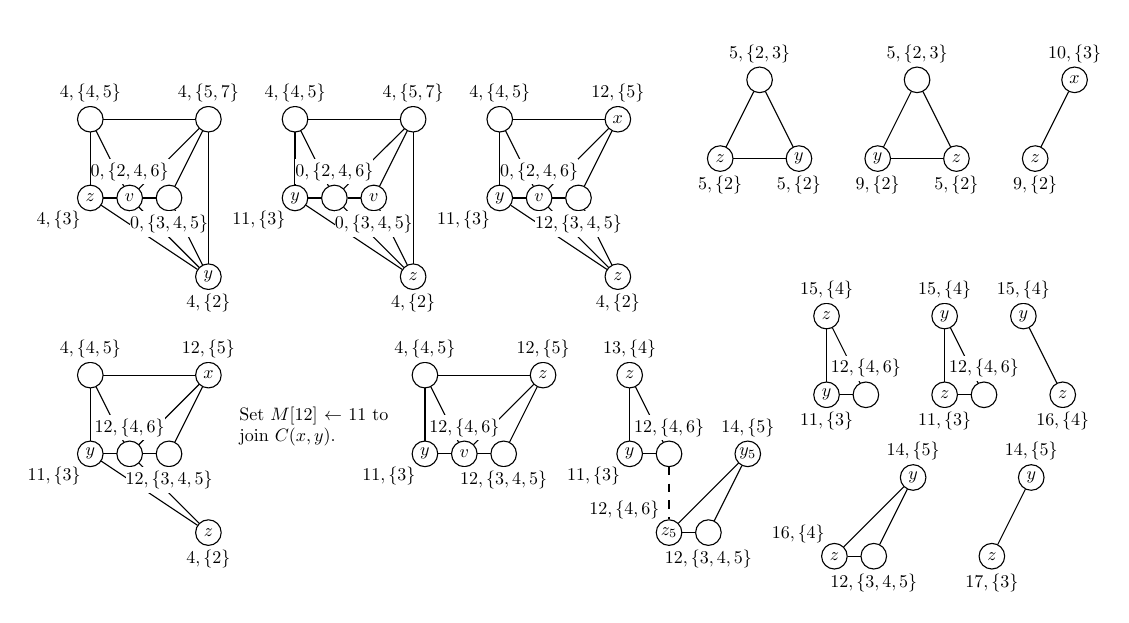
\begin{tikzpicture}
    \node[draw=none] at (0.0cm, 1.5cm) {};
    \node (u2) [label=below:${5,\{2\}}$] at (6.0cm, 0.0cm) {$z$};
    \node (v5) [label=above:${5,\{2,3\}}$] at (6.5cm, 1.0cm) {};
    \node (u3) [label=below:${5,\{2\}}$] at (7.0cm, 0.0cm) {$y$};

    \begin{pgfonlayer}{bg}
        \draw (u2) edge (u3);
        \draw (u2) edge (v5);
        \draw (u3) edge (v5);
    \end{pgfonlayer}{bg}

    \node (u2a) [label=below:${9,\{2\}}$] at (8.0cm, 0.0cm) {$y$};
    \node (v5a) [label=above:${5,\{2,3\}}$] at (8.5cm, 1.0cm) {};
    \node (u3a) [label=below:${5,\{2\}}$] at (9.0cm, 0.0cm) {$z$};

    \begin{pgfonlayer}{bg}
        \draw (u2a) edge (u3a);
        \draw (u2a) edge (v5a);
        \draw (u3a) edge (v5a);
    \end{pgfonlayer}{bg}
    
    \node (u2) [label=below:${9,\{2\}}$] at (10.0cm, 0.0cm) {$z$};
    \node (v5) [label=above:${10,\{3\}}$] at (10.5cm, 1.0cm) {$x$};

    \begin{pgfonlayer}{bg}
        \draw (u2) edge (v5);
    \end{pgfonlayer}{bg}

    \node (u1) [label=above:${4,\{4,5\}}$] at (-2.0cm, 0.5cm) {};
    \node (v1) [label=above:${4,\{5,7\}}$] at (-0.5cm, 0.5cm) {};
    \node (v2) [label=below left:${4,\{3\}}$] at (-2.0cm, -0.5cm) {$z$};
    \node (v3) [label=above:${0,\{2,4,6\}}$] at (-1.5cm, -0.5cm) {$v$};
    \node (v4) [label=below:${0,\{3,4,5\}}$] at (-1.0cm, -0.5cm) {};
    \node (u2) [label=below:${4,\{2\}}$] at (-0.5cm, -1.5cm) {$y$};

    \begin{pgfonlayer}{bg} 
        \draw (u1) edge (v2);
        \draw (v2) edge (u2);
        \draw (u1) edge (v1);
        \draw (u1) edge (v3);
        \draw (u2) edge (v3);
        \draw (u2) edge (v4);
        \draw (u2) edge (v1);
        \draw (v1) edge (v3);
        \draw (v1) edge (v4);
        \draw (v2) edge (v3);
        \draw (v3) edge (v4);
    \end{pgfonlayer}

    \node (u1a) [label=above:${4,\{4,5\}}$] at (0.6cm, 0.5cm) {};
    \node (v1a) [label=above:${4,\{5,7\}}$] at (2.1cm, 0.5cm) {};
    \node (v2a) [label=below left:${11,\{3\}}$] at (0.6cm, -0.5cm) {$y$};
    \node (v3a) [label=above:${0,\{2,4,6\}}$] at (1.1cm, -0.5cm) {};
    \node (v4a) [label=below:${0,\{3,4,5\}}$] at (1.6cm, -0.5cm) {$v$};
    \node (u2a) [label=below:${4,\{2\}}$] at (2.1cm, -1.5cm) {$z$};

    \begin{pgfonlayer}{bg} 
        \draw (u1a) edge (v2a);
        \draw (v2a) edge (u2a);
        \draw (u1a) edge (v1a);
        \draw (u1a) edge (v3a);
        \draw (u2a) edge (v3a);
        \draw (u2a) edge (v4a);
        \draw (u2a) edge (v1a);
        \draw (v1a) edge (v3a);
        \draw (v1a) edge (v4a);
        \draw (v2a) edge (v3a);
        \draw (v3a) edge (v4a);
    \end{pgfonlayer}

    \node (u1b) [label=above:${4,\{4,5\}}$] at (3.2cm, 0.5cm) {};
    \node (v1b) [label=above:${12,\{5\}}$] at (4.7cm, 0.5cm) {$x$};
    \node (v2b) [label=below left:${11,\{3\}}$] at (3.2cm, -0.5cm) {$y$};
    \node (v3b) [label=above:${0,\{2,4,6\}}$] at (3.7cm, -0.5cm) {$v$};
    \node (v4b) [label=below:${12,\{3,4,5\}}$] at (4.2cm, -0.5cm) {};
    \node (u2b) [label=below:${4,\{2\}}$] at (4.7cm, -1.5cm) {$z$};

    \begin{pgfonlayer}{bg} 
        \draw (u1b) edge (v2b);
        \draw (v2b) edge (u2b);
        \draw (u1b) edge (v1b);
        \draw (u1b) edge (v3b);
        \draw (u2b) edge (v3b);
        \draw (u2b) edge (v4b);
        \draw (v1b) edge (v3b);
        \draw (v1b) edge (v4b);
        \draw (v2b) edge (v3b);
        \draw (v3b) edge (v4b);
    \end{pgfonlayer}

    \node (u1c) [label=above:${4,\{4,5\}}$] at (-2.0cm, -2.75cm) {};
    \node (v1c) [label=above:${12,\{5\}}$] at (-0.5cm, -2.75cm) {$x$};
    \node (v2c) [label=below left:${11,\{3\}}$] at (-2.0cm, -3.75cm) {$y$};
    \node (v3c) [label=above:${12,\{4,6\}}$] at (-1.5cm, -3.75cm) {};
    \node (v4c) [label=below:${12,\{3,4,5\}}$] at (-1.0cm, -3.75cm) {};
    \node (u2c) [label=below:${4,\{2\}}$] at (-0.5cm, -4.75cm) {$z$};

    \begin{pgfonlayer}{bg} 
        \draw (u1c) edge (v2c);
        \draw (v2c) edge (u2c);
        \draw (u1c) edge (v1c);
        \draw (u1c) edge (v3c);
        \draw (u2c) edge (v3c);
        \draw (v1c) edge (v3c);
        \draw (v1c) edge (v4c);
        \draw (v2c) edge (v3c);
        \draw (v3c) edge (v4c);
    \end{pgfonlayer}

    \node[draw=none,text width=3.1cm] at (0.9cm, -3.4cm)
        {Set $M[12]\leftarrow11$ to join $C(x,y)$.};

    \node (u1d) [label=above:${4,\{4,5\}}$] at (2.25cm, -2.75cm) {};
    \node (v1d) [label=above:${12,\{5\}}$] at (3.75cm, -2.75cm) {$z$};
    \node (v2d) [label=below left:${11,\{3\}}$] at (2.25cm, -3.75cm) {$y$};
    \node (v3d) [label=above:${12,\{4,6\}}$] at (2.75cm, -3.75cm) {$v$};
    \node (v4d) [label=below:${12,\{3,4,5\}}$] at (3.25cm, -3.75cm) {};

    \begin{pgfonlayer}{bg} 
        \draw (u1d) edge (v2d);
        \draw (u1d) edge (v1d);
        \draw (u1d) edge (v3d);
        \draw (v1d) edge (v3d);
        \draw (v1d) edge (v4d);
        \draw (v2d) edge (v3d);
        \draw (v3d) edge (v4d);
    \end{pgfonlayer}

    \node (u1e) [label=above:${13,\{4\}}$] at (4.85cm, -2.75cm) {$z$};
    \node (v2e) [label=below left:${11,\{3\}}$] at (4.85cm, -3.75cm) {$y$};
    \node (v3e) [label=above:${12,\{4,6\}}$] at (5.35cm, -3.75cm) {};

    \node (v1ep) [label=above:${14,\{5\}}$] at (6.35cm, -3.75cm) {$y_5$};
    \node (v3ep) [label=above left:${12,\{4,6\}}$] at (5.35cm, -4.75cm) {$z_5$};
    \node (v4ep) [label=below:${12,\{3,4,5\}}$] at (5.85cm, -4.75cm) {};

    \begin{pgfonlayer}{bg} 
        \draw (u1e) edge (v2e);
        \draw (u1e) edge (v3e);
        \draw (v2e) edge (v3e);

        \draw (v3e) edge [dashed] (v3ep);

        \draw (v1ep) edge (v3ep);
        \draw (v1ep) edge (v4ep);
        \draw (v4ep) edge (v3ep);
    \end{pgfonlayer}

    \node (u1f) [label=above:${15,\{4\}}$] at (7.35cm, -2.0cm) {$z$};
    \node (v2f) [label=below:${11,\{3\}}$] at (7.35cm, -3.0cm) {$y$};
    \node (v3f) [label=above:${12,\{4,6\}}$] at (7.85cm, -3.0cm) {};

    \begin{pgfonlayer}{bg} 
        \draw (u1f) edge (v2f);
        \draw (u1f) edge (v3f);
        \draw (v2f) edge (v3f);
    \end{pgfonlayer}

    \node (u1f) [label=above:${15,\{4\}}$] at (8.85cm, -2.0cm) {$y$};
    \node (v2f) [label=below:${11,\{3\}}$] at (8.85cm, -3.0cm) {$z$};
    \node (v3f) [label=above:${12,\{4,6\}}$] at (9.35cm, -3.0cm) {};

    \begin{pgfonlayer}{bg} 
        \draw (u1f) edge (v2f);
        \draw (u1f) edge (v3f);
        \draw (v2f) edge (v3f);
    \end{pgfonlayer}

    \node (u1g) [label=above:${15,\{4\}}$] at (9.85cm, -2.0cm) {$y$};
    \node (v3g) [label=below:${16,\{4\}}$] at (10.35cm, -3.0cm) {$z$};

    \begin{pgfonlayer}{bg} 
        \draw (u1g) edge (v3g);
    \end{pgfonlayer}

    \node (v1fp) [label=above:${14,\{5\}}$] at (8.45cm, -4.05cm) {$y$};
    \node (v3fp) [label=above left:${16,\{4\}}$] at (7.45cm, -5.05cm) {$z$};
    \node (v4fp) [label=below:${12,\{3,4,5\}}$] at (7.95cm, -5.05cm) {};

    \begin{pgfonlayer}{bg} 
        \draw (v1fp) edge (v3fp);
        \draw (v1fp) edge (v4fp);
        \draw (v4fp) edge (v3fp);
    \end{pgfonlayer}

    \node (v1fp) [label=above:${14,\{5\}}$] at (9.95cm, -4.05cm) {$y$};
    \node (v4fp) [label=below:${17,\{3\}}$] at (9.45cm, -5.05cm) {$z$};

    \begin{pgfonlayer}{bg} 
        \draw (v1fp) edge (v4fp);
    \end{pgfonlayer}

    %\node (u1d) [label=above:${4,\{4,5\}}$] at (6.0cm, -2.75cm) {};
    %\node (v1d) [label=above:${12,\{5\}}$] at (7.5cm, -2.75cm) {$z$};
    %\node (v2d) [label=below left:${11,\{3\}}$] at (6.0cm, -3.75cm) {$y$};
    %\node (v3d) [label=above:${12,\{4,6\}}$] at (6.5cm, -3.75cm) {};
    %\node (v4d) [label=below:${12,\{3,4,5\}}$] at (7.0cm, -3.75cm) {};

    %\begin{pgfonlayer}{bg} 
    %    \draw (u1d) edge (v2d);
    %    \draw (u1d) edge (v1d);
    %    \draw (u1d) edge (v3d);
    %    \draw (v1d) edge (v3d);
    %    \draw (v1d) edge (v4d);
    %    \draw (v2d) edge (v3d);
    %    \draw (v3d) edge (v4d);
    %\end{pgfonlayer}

    %\node (u1d) [label=above:${4,\{4,5\}}$] at (0.6cm, -2.75cm) {};
    %\node (v1d) [label=above:${12,\{5\}}$] at (2.1cm, -2.75cm) {$z$};
    %\node (v2d) [label=below left:${11,\{3\}}$] at (0.6cm, -3.75cm) {$y$};
    %\node (v3d) [label=above:${12,\{4,6\}}$] at (1.1cm, -3.75cm) {};
    %\node (v4d) [label=below:${12,\{3,4,5\}}$] at (1.6cm, -3.75cm) {};

    %\begin{pgfonlayer}{bg} 
    %    \draw (u1d) edge (v2d);
    %    \draw (u1d) edge (v1d);
    %    \draw (u1d) edge (v3d);
    %    \draw (v1d) edge (v3d);
    %    \draw (v1d) edge (v4d);
    %    \draw (v2d) edge (v3d);
    %    \draw (v3d) edge (v4d);
    %\end{pgfonlayer}
\end{tikzpicture}
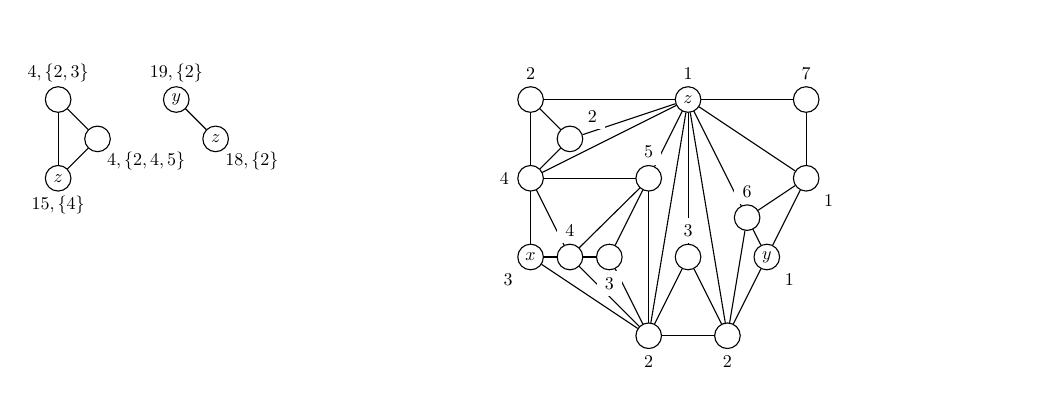
\begin{tikzpicture}
    \node[draw=none] at (-8.0cm, 2.25cm) {};
    \node[draw=none] at (4.0cm, 0.0cm) {};
    \node (u0r) [label=above:${4,\{2,3\}}$] at (-8.0cm, 1.5cm) {};
    \node (v0r) [label=below right:${4,\{2,4,5\}}$] at (-7.5cm, 1.0cm) {};
    \node (u1r) [label=below:${15,\{4\}}$] at (-8.0cm, 0.5cm) {$z$};

    \begin{pgfonlayer}{bg}
        \draw (u0r) edge (v0r);
        \draw (u1r) edge (v0r);
        \draw (u0r) edge (u1r);
    \end{pgfonlayer}

    \node (u0r) [label=above:${19,\{2\}}$] at (-6.5cm, 1.5cm) {$y$};
    \node (v0r) [label=below right:${18,\{2\}}$] at (-6.0cm, 1.0cm) {$z$};

    \begin{pgfonlayer}{bg}
        \draw (u0r) edge (v0r);
    \end{pgfonlayer}

    \node (z) [label=above:${1}$] at (0.0cm, 1.5cm) {$z$};
    \node (u0) [label=above:${2}$] at (-2.0cm, 1.5cm) {};
    \node (v0) [label=above right:${2}$] at (-1.5cm, 1.0cm) {};
    \node (u1) [label=left:${4}$] at (-2.0cm, 0.5cm) {};
    \node (v1) [label=above:${5}$] at (-0.5cm, 0.5cm) {};
    \node (v2) [label=below left:${3}$] at (-2.0cm, -0.5cm) {$x$};
    \node (v3) [label=above:${4}$] at (-1.5cm, -0.5cm) {};
    \node (v4) [label=below:${3}$] at (-1.0cm, -0.5cm) {};
    \node (u2) [label=below:${2}$] at (-0.5cm, -1.5cm) {};
    \node (v5) [label=above:${3}$] at (0.0cm, -0.5cm) {};
    \node (u3) [label=below:${2}$] at (0.5cm, -1.5cm) {};
    \node (v6) [label=below right:${1}$] at (1.0cm, -0.5cm) {$y$};
    \node (v7) [label=above:${6}$] at (0.75cm, 0.0cm) {};
    \node (u4) [label=below right:${1}$] at (1.5cm, 0.5cm) {};
    \node (u5) [label=above:${7}$] at (1.5cm, 1.5cm) {};

    \begin{pgfonlayer}{bg} 
        \draw (z) edge (u0);
        \draw (z) edge (u1);
        \draw (z) edge (u2);
        \draw (z) edge (u3);
        \draw (z) edge (u4);
        \draw (z) edge (u5);

        \draw (z) edge (v0);
        \draw (z) edge (v1);
        \draw (z) edge (v5);
        \draw (z) edge (v7);

        \draw (u0) edge (u1);
        \draw (u1) edge (v2);
        \draw (v2) edge (u2);
        \draw (u2) edge (u3);
        \draw (u3) edge (v6);
        \draw (v6) edge (u4);
        \draw (u4) edge (u5);

        \draw (u0) edge (v0);
        \draw (u1) edge (v0);
        \draw (u1) edge (v1);
        \draw (u1) edge (v3);
        \draw (u2) edge (v3);
        \draw (u2) edge (v4);
        \draw (u2) edge (v1);
        \draw (u2) edge (v5);
        \draw (u3) edge (v5);
        \draw (u3) edge (v7);
        \draw (u4) edge (v7);

        \draw (v1) edge (v3);
        \draw (v1) edge (v4);
        \draw (v2) edge (v3);
        \draw (v3) edge (v4);
        \draw (v6) edge (v7);
    \end{pgfonlayer}
\end{tikzpicture}

\caption{Algorithm~4.2 example continued.}
\label{F:hartman_impl_cont}
\end{center}
\end{figure}

\begin{algorithm}\label{A:hartman_impl}
    \textbf{Input:} Let $C$ be a cycle in a weakly triangulated plane graph $G$
    represented by augmented adjacency lists. Let $x,y,z\in C$ be
    vertices such that $z\in C(x,y)$.

    Let $L$ be an array of lists of colors
    such that for $v\in\{x,y,z\}$ the list $L[v]$ has length one,
    for $v\in C-\{x,y,z\}$ the list $L[v]$ has length two
    or three, and for $v\in \text{Int}(C)-C$ the list
    $L[v]$ has length three. Furthermore, for all $v\in C(x,z) - z$ assume
    that $L[v]$ does not contain the color in $L[z]$.

    Let $N$ be an array of pairs of
    references such that for each $v\in C$ the pair $N[v]=(r_1,r_2)$ has
    $r_1$ as a reference to the neighbor the immediately counter-clockwise
    from $v$
    around $C$, and $r_2$ as a reference
    to the neighbor immediately clockwise from $v$ around $C$.

    Let $S$ be an array of
    integers such that for all $v\in C(x,z)-z$ we have $S[v]=S[x]$ and for
    all vertices $v\in C-C(x,z)$ we have $S[v]\ne S[x]$. Furthermore, for all
    vertices $v\in C$ we $S[v]\ne 0$ and for all $v\in \text{Int}(C)-C$
    we have $S[v]=0$. Finally, let $M$
    be an array of integers such that for all vertices $v\in C(z,y)-z$ we have
    $M[S[v]]=S[y]$, and for all vertices $v\in C-C(z,y)$ we have $M[S[v]]\ne
    S[y]$.

    \textbf{Output:} Elements will be removed from the lists in $L$ such that
    for each $v\in\text{Int}(C)$ the list $L[v]$ consists of a single color. The
    coloring of $\text{Int}(C)$ corresponding to the remaining
    colors will be a path
    coloring $c$ such that $\text{deg}_c(x)\le1$, $\text{deg}_c(y)\le1$,
    and $\text{deg}_c(z)\le1$.

    \textbf{Procedure:} Let $N[z]=(r_1,r_2)$. Define the vertex $u_0$ to be
    the neighbor of $z$ corresponding to $r_1$, and define $v$ to be the
    neighbor of $z$ immediately clockwise from $u$.
    
    \textbf{Case 1 (Base Case):} If $r_1=r_2$ then $C=\{z,u_0\}$
    is a $2$-vertex path. If $u_0\ne x$ and $u_0\ne y$, remove color
    remaining in $L[z]$ from $L[u_0]$. If more than one color still remains in
    $L[u_0]$, remove arbitrary colors until a single color remains.

    \textbf{Case 2 (Recursive Step):} Suppose that $r_1\ne r_2$, and therefore $C$ is a cycle.

    \textbf{Case 2.1:} Suppose that $z=x$ and $u_0=y$. Make a recursive
    call after assigning $S[x]$ and $S[y]$ new unique marks and re-assigning
    $y'\leftarrow z$, $z'\leftarrow u_0$, $x'\leftarrow u_0$.

    \textbf{Case 2.2:} Suppose that $z=x$ and $u_0\ne y$. Make a recursive call after
    removing the color in $L[z]$ from $L[u_0]$,
    assigning $x'\leftarrow u_0$,
    $y'\leftarrow y$, $z'\leftarrow z$,
    and setting $S[u_0]$ to be a new unique mark.

    \textbf{Case 2.3:} Suppose that $z\ne x$ and $S[v]=0$, that is, $v\in
    \text{Int}(C)$. Assign $S[v]=S[x]$, remove the color in $L[z]$ from
    $L[v]$, and remove the edge $zu_0$ by adjusting
    $N[u_0]$ and $N[z]$. Make a recursive call and note that the new
    ``$u_0$'' in this call will be the current vertex $v$.

    \textbf{Case 2.4:} Suppose that $z\ne x$ and $S[v]=S[x]$, in other
    words $v\in C(x,z)$. Then we remove
    the edge $zu_0$ and make two
    recursive calls. The first call is with $x_1\leftarrow x$,
    $y_1\leftarrow y$, and $z_1\leftarrow z$, 
    but with $N[v]$ split at the edge $vz$ to only include neighbors clockwise
    from $z$. The second recursive call is 
    with $x_2,y_2,z_2$ all assigned equal to $v$ and $N[v]$ split at the edge
    $vz$ to contain only the neighbors of $v$ counterclockwise from $z$.

    \textbf{Case 2.5:} Suppose that $z\ne x$ and $M[S[v]]=S[y]$, in other words
    $v\in C(z,y)$. There are
    two different cases to consider.

    \textbf{Case 2.5.1:} Suppose that the color in $L[z]$ is in $L[v]$. We
    remove all other colors from $L[v]$, remove the edge $zu_0$, and make two
    recursive calls. The first call will be made with $x_1\leftarrow x$,
    $y_1\leftarrow y$, and $z_1\leftarrow v$, splitting $N[v]$ at the edge
    $vz$ to contain only neighbors counter-clockwise from $z$. The second
    recursive call will be made with $x_2\leftarrow v$, $y_2\leftarrow z$,
    and $z_2\leftarrow v$, splitting $N[v]$ at the edge $vz$ to include $z$
    and all neighbors clockwise from $z$.

    \textbf{Case 2.5.2:} Suppose that the color in $L[z]$ is not in $L[v]$.
    We remove the edge $zu_0$, assign $M[S[x]]=S[y]$, and make two recursive
    calls. The first call
    will be made with $x_1\leftarrow x$,
    $y_1\leftarrow y$, and $z_1\leftarrow x$, splitting $N[v]$ at the edge
    $vz$ to contain only neighbors counter-clockwise from $z$. The second
    recursive call will be made with $x_1\leftarrow v$, $y_1\leftarrow z$,
    and $z_1\leftarrow v$, splitting $N[v]$ at the edge $vz$ to include $z$
    and all neighbors clockwise from $z$.

    \textbf{Case 2.6:} Suppose that $z\ne x$ and $S[v]\ne 0$, but
    $S[v]\ne S[x]$ and $M[S[v]]\ne S[y]$, in other words $v\in C(y,x)-x-y$.
    First remove the color in $L[z]$ from $L[v]$, if it exists, and then remove
    arbitrary colors until $L[v]$ is of length one. Then remove the edge $zu_0$
    and make two recursive calls. The first call is made with $x_1\leftarrow x$,
    $y_1\leftarrow v$, and $z_1\leftarrow x$, splitting $N[v]$ at the edge $vz$
    to contain only neighbors counter-clockwise from $z$. The second call is
    made with $x_2\leftarrow v$, $y_2\leftarrow y$, and $z_2\leftarrow z$,
    splitting $N[v]$ at the edge $vz$ to contain $z$ and all neighbors clockwise
    from $z$.
\end{algorithm}

Every recursive case except for Case 2.1 and Case 2.2 removes an edge
from the representation and operates on one or two
strictly smaller subgraphs. In Case 2.1 a single recursive call is made
with an input that will not itself satisfy Case 2.1. In Case 2.2 a recursive
call is made with an input that will not itself satisfy Case 2.1 or Case 2.2.
Therefore the number of operations performed
is $\mathcal{O}(m)=\mathcal{O}(n)$.

Each operation performed is either integer arithmetic, an
array lookup, or a walk through a list of length three or less.
As each of these operations is constant time,
the algorithm has a time complexity of $\mathcal{O}(n)$.

\section{Experimental performance and parallelism}

A C implementation for both algorithms was run on randomly generated
triangulated plane graphs up to $10,000,000$ vertices. Benchmark timings
for both algorithms are shown below. Timings for a simple 
breadth-first search
(BFS) algorithm are also shown as baseline performance
for an algorithm that hits every half-edge.
All benchmarks
were run on an x86\_64 Intel N100 processor.

\begin{figure}[h]
\begin{center}
\begin{tabular}{r||r|r|r|r|r}
    & $n=10^3$  & $n=10^{4}$ & $n=10^{5}$ & $n=10^{6}$
        & $n=10^{7}$ \\
\hline
\hline
    BFS & %$1.66\cdot 10^{2}$ & $2.26\cdot 10^3$ &
    $2.39\cdot 10^{4}$ &
    $3.03\cdot 10^{5}$ &
    $3.85\cdot 10^{6}$ & $1.16\cdot 10^{8}$ &
    $1.48\cdot 10^{9}$ \\
\hline
    Poh & % $4.28\cdot 10^{2}$ & $6.48\cdot 10^3$ &
    $7.10\cdot 10^{4}$ & $8.12\cdot 10^{5}$ &
    $1.00\cdot 10^{7}$ & $2.16\cdot 10^{8}$ &
    $2.69\cdot 10^{9}$ \\
\hline
    Poh (3 threads) & % $4.28\cdot 10^{2}$ & $6.48\cdot 10^3$ &
    $1.25\cdot 10^{5}$ & $1.17\cdot 10^{6}$ &
    $1.20\cdot 10^{7}$ & $1.47\cdot 10^{8}$ &
    $1.69\cdot 10^{9}$ \\
\hline
    Hartman & % $7.62\cdot 10^{2}$ & $9.30\cdot 10^3$ &
    $1.04\cdot 10^{5}$ & $1.23\cdot 10^{6}$ &
    $2.93\cdot 10^{7}$ & $6.44\cdot 10^{8}$ &
    $7.73\cdot 10^{9}$ \\
\hline
    Hartman (3 threads) & % $7.62\cdot 10^{2}$ & $9.30\cdot 10^3$ &
    $2.18\cdot 10^{5}$ & $2.19\cdot 10^{6}$ &
    $3.30\cdot 10^{7}$ & $5.84\cdot 10^{8}$ &
    $6.71\cdot 10^{9}$ \\
\end{tabular}
    \caption{Benchmarks (ns / graph) for
    Algorithm~\ref{A:poh_linear} and
    Algorithm~\ref{A:hartman_impl}.}
\end{center}
\end{figure}

The Poh and Hartman-\v{S}krekovski algorithms color graphs by operating on
weakly-triangulated subgraphs that are disjoint except for vertices on their
respective outer faces. Therefore it is possible to maintain a stack of
independent recursive frames and have a pool of threads operate on these frames
in parallel.

In the case of Poh's algorithm this can be achieved trivially as each
frame writes only to vertices interior to the outer face. The
algorithm may use a shared mutex or spin-lock guarded stack of frames from
which all threads will push and pop frames.
If no frames are
available, a thread must idle until either a new frame is pushed to the stack or
all other threads are idle.

Benchmarks showed the best performance improvements for Poh's algorithm when
using three threads to color plane graphs on the order of $10^6$ vertices
or more. 

The Hartman-\v{S}krekovski algorithm is tricker to adapt to
parallel execution. The first diffuculty to consider is that certain recursive
frames are
dependent on each other: the recursive calls made in
Algorithm 4.2 cannot be re-ordered, with the exception of
in Case 2.4.1 and Case 2.5. For a concrete example,
in Figure~\ref{F:hartman_impl} the first recursive
frame produced cannot start until the vertex $z_0$ has it's list $L[z_0]$
reduced from $\{4,5\}$ down to $\{4\}$, which does not happen
until much later in Figure~\ref{F:hartman_impl_cont}. A smaller, but no less important detail is that
if two threads ever use the
same face mark then we risk data races against the array $M$.

The first hurdle of dependent frames can be solved by maintaining a shared
lock-guarded object pool
of frames and a stack of frame references. Recursive frames are added to the
pool when they appear in the usual course of the algorithm, but
only pushed to the stack when they
are ready to be colored. For each vertex $v$ we maintain an optional reference
to a frame that will become ready when $v$ has been colored. Frames in the
object pool will store intrusive linked list references so that multiple frames
can await the coloring of a single vertex. Whenever a vertex $v$ is
colored we simply walk the linked list of frames that were waiting on $v$
and push references to those frames onto the stack.

The issue of unique marks can be solved by using an atomic mark counter
shared between all threads. Contention can be minimized by having
threads reserve marks in large chunks, rather than performing an
atomic fetch-add operation for each new mark.

Benchmarks for the parallelized Hartman-\v{S}krekovski algorithm showed
the best performance
benefits when using three threads to color plane graphs on the order
of $10^6$ vertices or more.
The gains observed were less significant than those observed for the
Poh algorithm, but that was to be expected as the recursive frames are often
dependent and thread coordination is more complicated.

%    If $z\ne y$, define $u$ to be the closest vertex to $y$ in $C(z,y)-z$
%    that is adjacent to $z$. Note that $u$ is either
%    the vertex immediately clockwise from $z$ around $C$ or a cut-vertex of
%    $G-z$, and it may be that $u=y$. Otherwise, define $u=z$.
%
%    We define a new list function
%    $L'$ such that
%    \begin{align*}
%        L'(v)&=\{\ c(z)\ \} \text{ if } v=u\text{ and } c(v)\in L(u);; \\
%        L'(v)&=L(v)\setminus\{\ c(z)\ \} \text{ otherwise.}
%    \end{align*}
%    Note that if $v\in G$ is not adjacent to $z$ then $L'(v)=L(v)$, in
%    particular $L'(v)=L(v)$ except for vertices on the outer face of $G-z$.
%    Moreover, $L'(v)=L(v)$ for all $v\in C(x,z)-z$. We will show that for each
%    $2$-connected component of $G-z$ there we can select $x',y',z'$ on the outer
%    face that together with the list assignment $L'$ satisfy the requirements of
%    the algorithm. We will also show that the resulting path $L'$-choosings
%    of each subgraph agree on shared vertices and combine form a path
%    $L$-choosing of $G$.
%
%    \textbf{Case 2.1:} Suppose that $z$ has exactly two neighbors in
%    $C$, and therefore $G-z$ is $2$-connected. Let $C'$ be the outer face of
%    $G-z$.
%    
%    \textbf{Case 2.1.1:} Suppose that $x=y=z$. Define $x'$ and $y'$
%    to be the
%    vertices immediately counter-clockwise and clockwise from $z$ in $C$,
%    respectively. Define $z'=x'$. Note that $|L(x')|\ge 1$, $|L(y')|\ge1$, and
%    $|L(u)|\ge 2$ for all $u\in C'-x'-y'$. Thus we may recursively color
%    $\text{Int}(C')$ from list assignment $L'$. No vertex in $G-z$
%    adjacent to $z$ in $G$ will receive the color $c(z)$, thus the path
%    $L'$-choosing
%    of $G-z$ extends to an path $L$-list coloring of $G$.
%
%    \textbf{Case 2.1.2:} Suppose that $x=z$, $z\ne y$. Define $x'$
%    to be the vertex immediately counter-clockwise to $x$ around $C'$.
%    Let $u$ be the vertex immediately clockwise to $z$ around $C$. If
%    
%    If $x=v$ let $H$ be the first $2$-connected component of $G-v$
%    counter-clockwise from $v$, otherwise let $H$ be the $2$-connected
%    component containing $x$. Define a new list assignment $L'$ such that
%    $L'(u)=L(u)-L(v)$.
%    from $x$ to $v$ around $C$. Note that each $u\in C(x,v)-v$ such that $uv\in
%    E(G)$ will be a cut vertex of 
%\end{algorithm}
%
%\begin{algorithm}[Hartman 1997, \v{S}krekovski 1999]\label{A:hartman3}
%\textbf{Input:} A cycle $C$ in a triangulated plane graph $G$, a pair of
%vertices $x,y\in C$ (not necessarily distinct), and function
%$L:V(G)\to P_{<\aleph_0}(\mathbb{N})$ that assigns a finite set of
%``colors'' to each vertex such that
%\begin{align*}
%    |L(v)| &\ge 1 \text{ for } v\in\{x,y\} \\
%    |L(v)| &\ge 2 \text{ for } v\in V(C)\setminus\{x,y\} \\
%    |L(v)| &\ge 3 \text{ for } v\in V(G)\setminus V(C).
%\end{align*}
%\textbf{Output:} A path $3$-coloring $c:V(G)\to\mathbb{N}$ of $G$ such that
%$c(v)\in L(v)$ for all $v\in V(G)$.
%
%\textbf{Step 1:} Define $c(x)$ and $c(y)$ to be a color in their
%    respective
%    list. Let $C(x,y)$ be the set of vertices between $x$ and $y$ clockwise
%    along $C$, including $x$ and $y$. We will construct an induced path $P$ that
%    starts at $x$ and consists only of vertices $v\in C(x,y)$ such that
%    $c(x)\in L(v)$. Start with $P={x}$. Let $u$ be the last vertex added to $P$
%    and consider the neighbor $v$ of $x$
%    that is furthest clockwise towards $y$ in $C(x,y)$. If $c(x)\in L(v)$, then
%    add $v$ and the edge $uv$ to $P$ and repeat, otherwise we have finished
%    constructing $P$.
%
%\textbf{Step 2:} Define a new color assignment
%    $L'$ such that
%    \begin{align*}
%        L'(v)&=L(v)\setminus\{\ c(x)\ \} \text { if } v
%            \text{ has a neighbor in } P \\
%        L'(v)&=L(v)\text{ otherwise.}
%    \end{align*}
%    Let $H$ be a $2$-connected components of $G-P$. Let $v_1,v_2,v_3\in H\cap C$
%    such that $v_2$ is in the path from $v_1$ to $v_3$ clockwise along $C$.
%    Observe that $v_2$ has a neighbor in $P$ when considered as a vertex of $G$
%    then any path $v_1$ to $v_3$ must pass through $v_2$. So it must
%    be that $v_2=v_1$ or
%    $v_2=v_3$. Thus there are at most two vertices in $H\cap C$ that had
%    neighbors in $P$.
%
%    Note that if $v\in H$ is not
%    on the outer face of $H$ then $L'(v)=L(v)$ since $v$ could not have had a
%    neighbor in $P$. If $v\in H$ is on the outer face then if
%    $v\in H-C$ it must be that $|L'(v)|\ge 2$, and if $v\in H\cap C$ it must be
%    that $|L'(v)|\ge 1$. We may therefore recursively apply
%    Algorithm~\ref{A:hartman3} to path $L'$ list color each $2$-connected
%    component $H$ of $G-P$.
%
%    Suppose that $u\in G-P$ is contained in at least two $2$-connected
%    component $H_1,H_2$. Let $u\in H_1$ and $v\in H_2$
%
%    We may proceed to color the $2$-connected components of $G-P$ moving
%    clocwise from $x$ along $C$ above $P$ and counter-clockwise
%    from $x$ below $P$.
%\end{algorithm}


\begin{thebibliography}{99}

\bibitem{BoMy2004}
J.~Boyer and W.~Myrvold, On the cutting edge: simplified $O(n)$ planarity by edge
addition,
\textit{J. Graph Algorithms Appl.}
\textbf{8} (2004),
241--273.

\bibitem{BrMy1985}
I.~Broere and C.~M.~Mynhardt,
Generalized colorings of outerplanar and planar graphs,
\textit{Graph theory with applications to algorithms and computer science}
 (Kalamazoo, Mich., 1984),
pp.~151--161,
Wiley-Intersci. Publ., Wiley, New York, 1985.

\bibitem{Bro2017}
A.~Bross,
\textit{Implementing path coloring algorithms on planar graphs},
Masters Project,
University of Alaska,
2017,
available from\hfil\break
\texttt{http://github.com/permutationlock/path\_coloring\_bgl}.

\bibitem{ChHa2017prep}
G.~G.~Chappell and C.~Hartman,
Path choosability of planar graphs,
in preparation.

\bibitem{ChKr1969}
G.~Chartrand and H.~V.~Kronk,
The point-arboricity of planar graphs,
\textit{J. London. Math. Soc.}
\textbf{44} (1969),
612--616.

\bibitem{God1991}
W.~Goddard,
Acyclic colorings of planar graphs,
\textit{Discrete Math.}
\textbf{91} (1991), no. 1,
91--94.

\bibitem{Har1997}
C.~M.~Hartman,
\textit{Extremal Problems in Graph Theory},
Ph.D. Thesis,
University of Illinois,
1997.

\bibitem{Poh1990}
K.~S.~Poh,
On the linear vertex-arboricity of a planar graph,
\textit{J. Graph Theory}
\textbf{14} (1990), no. 1,
73--75.

\bibitem{Skr1999}
R.~\v{S}krekovski,
List improper colourings of planar graphs,
\textit{Combin. Probab. Comput.}
\textbf{8} (1999), no. 3,
293--299.

\bibitem{Wes2000}
D.~B.~West,
\textit{Introduction to Graph Theory, 2nd ed.},
Prentice Hall,
Upper Saddle River, NJ,
2000.

\end{thebibliography}

\end{document}

